\documentclass[a4paper, 12pt]{scrbook}
\pdfpagewidth\paperwidth
\pdfpageheight\paperheight
\usepackage{hyperref}
\hypersetup{
	colorlinks=true,
	linkcolor=black,
	filecolor=magenta,      
	urlcolor=black,
	citecolor=black,
}
\urlstyle{same}
\usepackage[italian]{babel}
\usepackage[utf8]{inputenc}
\usepackage[T1]{fontenc}
\usepackage{geometry}
\geometry{a4paper, top=3cm, bottom=3cm, left=3cm, right=3cm}
\usepackage{setspace}
\onehalfspacing
\usepackage{graphicx}
\usepackage[font=small,labelfont=bf]{caption}
\usepackage{textcomp}
\usepackage{bm}
\usepackage{subfigure}
\usepackage{amsmath}
\usepackage{colortbl}
\usepackage[table]{xcolor}
\definecolor{mygreen}{RGB}{60,179,113}
\usepackage{multirow}
\setlength{\parskip}{0em}
\usepackage[binary-units = true]{siunitx}
\usepackage{nicefrac}
\usepackage{verbatim}
\usepackage{array}
\usepackage{amssymb}
\usepackage{textcomp}
\usepackage{longtable}
\usepackage{bm}
\usepackage{nicematrix}
\usepackage{adjustbox}
\usepackage{rotating}
\usepackage{pdfpages}
\usepackage{placeins}
\usepackage{float}
\usepackage{natbib}

\usepackage{caption}
\captionsetup[figure]{format=plain}
\captionsetup[table]{format=plain}

\begin{document}
	
	\pagenumbering{Roman}
	\setcounter{page}{1}
	\tableofcontents
	\listoffigures
	\listoftables
	
	% \cite{paper_EM_algorithm}
	% \cite{paper_FDA_toolbox}
	% \cite{paper_GPM}
	% \cite{paper_f_HDGM}
	% \cite{paper_TS_book}
	% \cite{paper_GRASPA}
	% \cite{paper_HDGM}
	% \cite{paper_bike_sharing_e_popolazione}
	% \cite{paper_bike_sharing_e_ambiente}
	% \cite{paper_bike_sharing_e_meteo}
	% \cite{paper_bike_sharing_Otto}
	% \cite{paper_bike_sharing_e_covid}
	
	\mainmatter
	\addchap[Introduzione]{Introduzione}

I modelli spazio-temporali sono un fondamentale strumento concettuale utilizzato in una vasta gamma di discipline scientifiche per comprendere e analizzare fenomeni che si sviluppano nello spazio e nel tempo. Questi sistemi statistici forniscono un framework indispensabile per la descrizione e la predizione di eventi fisici, sociali, economici e naturali, permettendo agli studiosi di esplorare le relazioni tra le varie variabili in contesti complessi.
\par L'importanza di tali modelli nella vita quotidiana è evidente in molteplici contesti. Ad esempio, nel campo delle scienze ambientali, consentono di monitorare e modellare i cambiamenti climatici, le variazioni negli ecosistemi e la diffusione di inquinanti. Nell'ambito della pianificazione urbana, invece, sono utilizzati per ottimizzare la distribuzione delle risorse e dei servizi, migliorando la qualità della vita nelle città. Inoltre, nel settore dei trasporti, contribuiscono a ottimizzare le reti di trasporto e a gestire il traffico in tempo reale, riducendo congestioni e tempi di percorrenza.
\par Uno dei modelli spazio-temporali proposti in letteratura è il \textit{Functional Hidden Dynamic Geostatistical Model} (\textit{f-HDGM})~\citep{paper_f_HDGM}. Esso, oltre a essere un modello funzionale, è anche \textit{state-space}; una variabile latente consente di rappresentare e modellare fenomeni non direttamente osservabili, ma che influenzano il comportamento del sistema. Si ipotizzi, per esempio, di voler descrivere la concentrazione di anidride carbonica rilevata nel tempo da una stazione di misura in funzione dell'umidità relativa. Probabilmente il loro legame cambia a seconda dell'ora del giorno, un effetto che, inoltre, potrebbe mutare da un giorno all'altro; infatti, non è detto che l'umidità relativa descriva la concentrazione dell'inquinante in oggetto sempre nello stesso modo, sia in estate che in inverno, in tutti i punti spaziali. Per modellare questa variabilità spazio-temporale, non direttamente osservabile dai dati, subentra la componente latente.
\par Uno dei limiti del modello f-HDGM è l'impossibilità di tener conto dell'interazione che potrebbe esistere tra punti di misura. Si prenda come esemplificazione il potenziale di mercato spaziale; esso rappresenta il volume di vendite previsto quando un determinato prodotto viene commercializzato in un'area di scambio. Le vendite sono previste essere elevate se un negozio viene aperto in una posizione caratterizzata da un alto potenziale di mercato spaziale, mentre si prevede una loro riduzione ove il potenziale mercato risulta essere basso. Ad esempio, se si ipotizzasse di aprire un nuovo punto vendita nelle vicinanze di altri negozi concorrenti ugualmente attrattivi\footnote{la decisione da parte del cliente di scegliere un negozio piuttosto che un altro è oggettiva, ossia non è influenzata da aspetti personali. Di conseguenza, si assume che l'unico fattore decisionale sia la distanza.}, allora essi si spartirebbero la domanda in quell'area; ciò si riflette in un basso potenziale. Al fine di ottenere una stima riguardo al volume degli scambi commerciali, la valutazione del potenziale di mercato spaziale emerge come un aspetto cruciale. 
\par La reciproca influenza tra i negozi, dove il volume delle vendite di ciascun punto è influenzato dalla presenza degli altri, rende imprescindibile considerare tale interazione al fine di stimare correttamente il potenziale di mercato spaziale. Da tale necessità deriva l'obiettivo di questo lavoro: estendere il modello f-HDGM affinché tenga conto anche di quest'aspetto.
\par Dopo aver introdotto nel primo capitolo il concetto di analisi funzionale e di stima Expectation-Maximization (EM), nel secondo e nel terzo si entra in medias res illustrando prima l'estensione del modello e poi le formule di stima dei suoi parametri. Nel quarto capitolo, invece, le nozioni teoriche vengono applicate a un caso di studio riguardante il fenomeno del bike sharing in una metropoli statunitense. Infine, il quinto capitolo chiude il lavoro traendo le considerazioni finali e illustrando i possibili sviluppi futuri. 
	\chapter[Il modello f-HDGM e l'algoritmo EM]{Introduzione all'analisi funzionale di dati spazio-tempo tramite il modello f-HDGM e cenni sull'algoritmo EM}

In questo primo capitolo, dopo aver presentato il concetto di analisi funzionale (\textit{Functional Data Analysis}, o \textit{FDA}), viene illustrato il modello spazio-temporale oggetto dell'estensione presentata in questo studio, ossia il \textit{Functional Hidden Dynamic Geostatistical Model} (o \textit{f-HDGM}). Infine, vengono fornite alcune nozioni per comprendere il funzionamento e, in primis, l'idea su cui si basa l'\textit{algoritmo EM}.

\section[Cenni sull'analisi funzionale dei dati]{Cenni sull'analisi funzionale dei dati}

\subsection[Differenza tra statistica inferenziale e analisi funzionale]{Differenza tra statistica inferenziale e analisi funzionale}
Fornito un campione di dati $D = (x_1, y_1), (x_2, y_2)\dots (x_N, y_N)$ e un modello $y = f(x, \boldsymbol{\theta}_0)$, l'obiettivo della statistica inferenziale è quello di stimare i parametri $\boldsymbol{\theta}_0$ andando a minimizzare una funzione di costo $J(\boldsymbol{\theta})$, ossia individuare la combinazione di valori stimati dei parametri $\boldsymbol{\hat{\theta}}_N$ tale che $\boldsymbol{\hat{\theta}}_N = \text{arg}\,\min\limits_{\boldsymbol{\theta}} J(\boldsymbol{\theta}, D)$. La funzione di costo cambia a seconda del modello da identificare e della tipologia di stima che viene utilizzata, per esempio OLS o MLE. Inoltre, non sempre è possibile risolvere il problema di minimo in forma chiusa\footnote{impiego di un'espressione matematica, esente da variabili libere, per calcolare il valore del parametro incognito. La ricerca iterativa dell'ottimo tramite un algoritmo non è necessaria.}; spesse volte è necessario ricorrere a tecniche di ottimizzazione numerica, in particolare quando la funzione $J(\boldsymbol{\theta})$ non è convessa. \par Nell'analisi funzionale, invece, l'oggetto della stima non è $\boldsymbol{\theta}$, ma la funzione $f$ continua. Le spline sono una delle classi di funzioni più utilizzate in FDA; la possibilità di regolare  la \textit{smoothness} rende loro facilmente generalizzabili.

\subsection[Basi di Fourier]{Basi di Fourier}
Le basi di Fourier sono una classe di spline che viene impiegata per descrivere segnali periodici. Il modello che il toolbox FDA per MATLAB~\cite{paper_FDA_toolbox} implementa è:
\[
	y(t) = \sqrt{2f}\cdot w(t)\\;
\]
\[
	w(t) = \frac{a_0}{\sqrt{2}} + \mathbf{a}_1\cdot \mathbf{k}_1(t)^\top +\dots + \mathbf{a}_i\cdot \mathbf{k}_i(t)^\top + \dots + \mathbf{a}_n\cdot \mathbf{k}_n(t)^\top;
\]
\[
	\mathbf{a}_i\in\mathbb{R}^{1\times2} =
	\begin{bmatrix}
		a_{i, \sin} & a_{i, \cos}
	\end{bmatrix};
\]
\[
	\mathbf{k}_i(t)\in\mathbb{R}^{1\times 2} =
	\begin{bmatrix}
		\sin\left(i\cdot\omega_0\cdot t\right) & \cos\left(i\cdot\omega_0\cdot t\right)
	\end{bmatrix}.
\]
$f$ è la frequenza, $n$ indica il numero di armoniche\footnote{il numero di basi è $n\cdot 2 + 1$.}, $\omega_0 = 2\pi\cdot f$ rappresenta la pulsazione dell'armonica fondamentale, mentre $a_0, a_1,\dots a_n$ sono i coefficienti combinatori. Oltre alla parte costante, ciascuna funzione seno e coseno costituisce una base. Una volta scelto il valore di $n$ a seconda del livello di complessità desiderato, l'obiettivo dell'analisi funzionale è quello di calcolare i coefficienti. Nelle figure \ref{esempi_Fourier} e \ref{esempio_Fourier_coef_non_unitari} sono riportati degli esempi sia di funzioni base sia di spline\footnote{combinazione lineare di basi di Fourier.}.

\begin{figure}[htp]
	\centering
	\subfigure[]{\label{}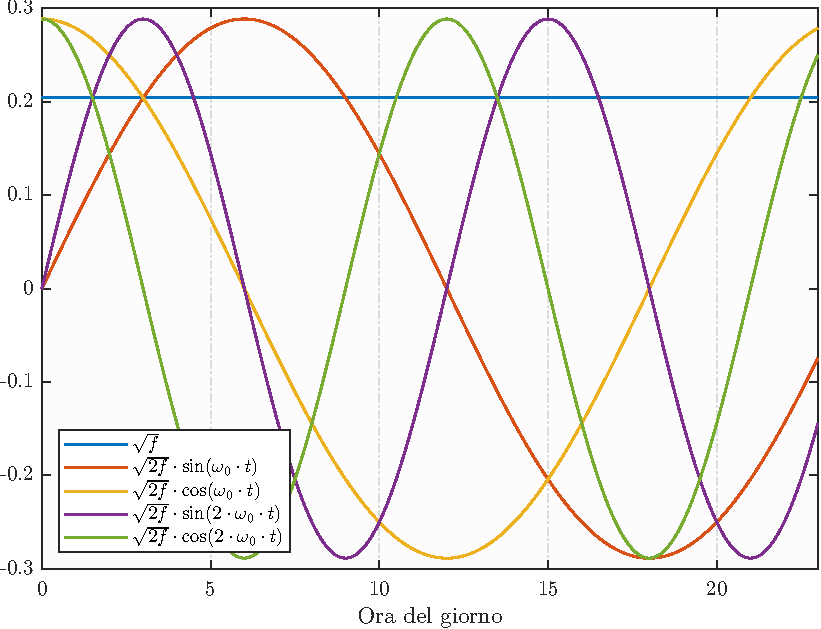
\includegraphics[height=158px]{Immagini/1. Modello base/Basi Fourier}}\quad
	\subfigure[]{\label{}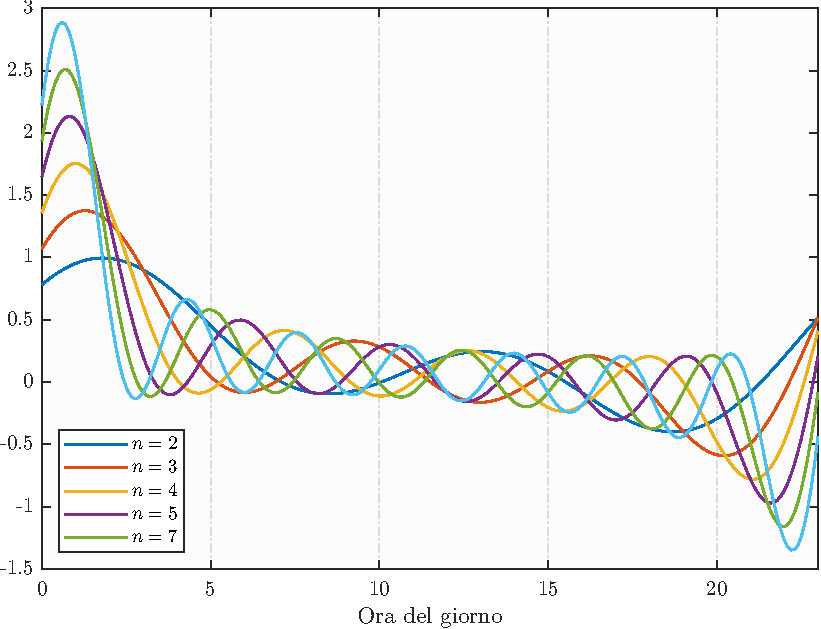
\includegraphics[height=158px]{Immagini/1. Modello base/Spline Fourier}}
	\caption[Confronto tra funzioni base con $n=2$ e tra diverse spline di Fourier]{confronto tra funzioni base con $n=2$ (a) e tra diverse spline di Fourier (b) i cui coefficienti combinatori sono unitari. Da notare come all'aumentare di $n$ la funzione risultante tenda al livello basso di un'onda quadra.}
	\label{esempi_Fourier}
\end{figure}
\begin{figure}[htp]
	\centering
	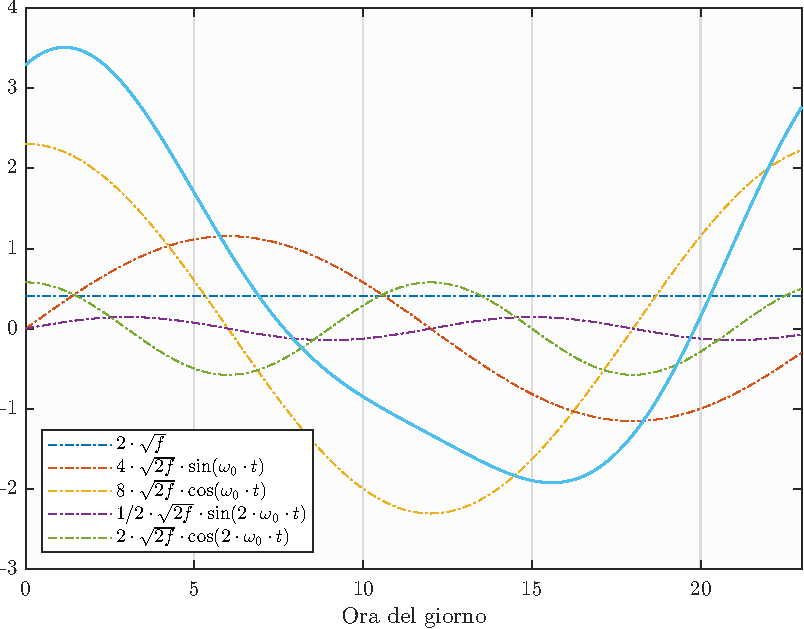
\includegraphics[height=180px]{Immagini/1. Modello base/Spline Fourier con coefficienti non unitari}
	\caption[Esempio di spline di Fourier con $n=2$ i cui coefficienti combinatori sono diversi da \num{1}]{esempio di spline di Fourier (in azzurro) con $n=2$ i cui coefficienti combinatori sono diversi da \num{1}. Nello specifico: $a_0 = 2$, $a_{1,\sin} = 4$, $a_{1,\cos} = 8$, $a_{2,\sin} = 1/2$ e $a_{2,\cos} = 2$.}
	\label{esempio_Fourier_coef_non_unitari}
\end{figure}

\subsection[Analisi funzionale e dati spazio-tempo]{Analisi funzionale e dati spazio-tempo}
Si ipotizzi di avere a disposizione i dati di temperatura acquisiti da due sensori collocati in due punti distinti di una stanza, ossia $T(\mathbf{s}_1, t)$ e $T(\mathbf{s}_2, t)$. La correlazione spaziale esistente tra punti, in aggiunta all'autocorrelazione temporale, può essere impiegata per prevedere la temperatura in una terza posizione $\mathbf{s}_3$ all'istante di tempo $t_0$. Per eseguire questa operazione utilizzando un modello non funzionale, tuttavia, è necessario conoscere sia $T(\mathbf{s}_1, t_0)$ sia $T(\mathbf{s}_2, t_0)$, una condizione che potrebbe non verificarsi sempre nel caso in cui i due sensori siano \textit{asincroni}. A questo punto sarebbe necessario ricorrere a una delle tecniche di interpolazione note in letteratura per stimare i dati mancanti, strategie che inevitabilmente introducono del rumore nel modello. \par L'indipendenza dalla sincronia e dalla continuità delle serie storiche rendono i modelli funzionali particolarmente adatti a risolvere situazioni di questa natura; una volta stimata la funzione $f$, infatti, è possibile utilizzarla per effettuare predizioni in qualsiasi punto e in qualsiasi istante.

\section[Il modello f-HDGM]{Il modello f-HDGM}
Il Functional Hidden Dynamic Geostatistical Model è stato illustrato in un articolo scientifico pubblicato sul Journal of Statistical Software nel settembre del \num{2021}, un paper finalizzato a presentare, oltre al modello, anche D-STEM v2, un software il cui scopo è stimare tramite l'algoritmo EM una serie di modelli spazio-temporali~\cite{paper_f_HDGM}.

\subsection[Equazioni del modello]{Equazioni del modello}
\label{equazioni_modello_base}
Sia $\mathbf{s} = (s_{lon}, s_{lat})^\top$ un generico punto spaziale sulla sfera terrestre $\mathbb{S}^2$ e $t\in\mathbb{N}$ un indice temporale discreto. Si assume che la funzione di interesse $f(\mathbf{s}, l, t)$, con dominio $\mathcal{L}=[l_1, l_q]\subset\mathbb{R}$, possa essere osservata in ogni $(\mathbf{s}, t)$ ed $l\in \mathcal{L}$ attraverso delle misurazioni rumorose $y(\mathbf{s}, l, t)$ che seguono il seguente modello matematico:
\begin{equation}
	y(\mathbf{s}, l, t) = f(\mathbf{s}, l, t) + \epsilon(l);
	\label{eq_rumore_uscita}
\end{equation}
\begin{equation}
	f(\mathbf{s}, l, t) = \mathbf{x}(\mathbf{s}, l, t)^\top\cdot\boldsymbol{\beta}(l) + \Phi_z(l)^\top\cdot\mathbf{z}(\mathbf{s}, t);
	\label{eq_comp_det}
\end{equation}
\begin{equation}
	\mathbf{z}(\mathbf{s}, t) = G\cdot \mathbf{z}(\mathbf{s}, t-1) + \boldsymbol{\eta}(\mathbf{s}, t).
	\label{eq_comp_lat}
\end{equation}
Prima di entrare in medias res, è bene introdurre la nomenclatura che successivamente verrà utilizzata per definire nel modello le dimensioni degli oggetti matriciali e vettoriali:
\begin{itemize}
	\item $n$ indica il numero di posizioni spaziali (o punti di misura) $\mathbf{s}\in\mathbb{R}^2$ prese in esame;
	\item $q$ rappresenta la dimensione del dominio (funzionale) $\mathcal{L}$ rappresentante l'alta frequenza. Se, per esempio, tramite l'indice discreto $h$ ci si vuole riferire all'ora del giorno, allora $q=24$ (da $0$ a $23$ con risoluzione $1$);
	\item $T$ indica il numero di campioni in bassa frequenza, ad esempio i giorni. In assenza di dati mancanti, il singolo campione è costituito da $n\cdot q = N$ osservazioni (per ognuna delle $n$ posizioni spaziali sono note tutte le $q$ rilevazioni della variabile $y$, una per ogni ora del giorno);
	\item $b$ rappresenta il numero di variabili esplicative, ovvero $|\boldsymbol{\beta}(l)| = b$;
	\item infine, $n_\epsilon$, $n_\beta$ ed $n_z$ indicano il numero di funzioni base utilizzate per modellare rispettivamente $\sigma_\epsilon (l)$, ogni $\beta(l)$ e $\Phi(l)$ per $\mathbf{z}(\mathbf{s}, t)$.
\end{itemize}
Da sottolineare che attualmente non esiste una versione multi-variata\footnote{$\mathbf{y}(\mathbf{s}, l, t)\in\mathbb{R}^{p\times 1}$, con $p>1$.} dell'f-HDGM.

\subsection[Rumore sull'uscita]{Rumore sull'uscita}
Nell'equazione \ref{eq_rumore_uscita}, $\epsilon (l)\in\mathbb{R}$ è una variabile causale con distribuzione gaussiana avente media nulla ($\mu_\epsilon = 0$), indipendente sia nello spazio sia nel tempo. La sua varianza $\sigma_\epsilon(l)$ è \textit{eteroschedastica}\footnote{dato un campione di variabili casuali, al suo interno esistono delle sotto-popolazioni che hanno diverse varianze.} nel dominio $\mathcal{L}$; essa è modellata nel modo seguente:
\[
	\log(\sigma_\epsilon(l)) = \Phi(l)^\top\cdot\mathbf{c}_\epsilon.
\]
$\Phi_z(l)\in\mathbb{R}^{n_\epsilon\times 1}$ sono le $n_\epsilon$ funzioni base valutate in $l$, mentre $\mathbf{c}_\epsilon\in\mathbb{R}^{n_\epsilon\times 1}$ i rispettivi coefficienti combinatori da stimare. \par La finalità della modellazione funzionale della varianza consiste nell'adattare il livello di incertezza in base a vari fattori, come ad esempio l'orario del giorno. Ciò è dovuto al fatto che il numero di osservazioni disponibili per ciascuna delle $q$ fasce orarie non rimane costante.

\subsection[Componente deterministica]{Componente deterministica}
Nell'equazione \ref{eq_comp_det}, $\mathbf{x}(\mathbf{s}, l, t)\in\mathbb{R}^{b\times 1}$ è un vettore di variabili esplicative, i cui coefficienti moltiplicativi $\boldsymbol{\beta}(l) = (\beta_1(l),\dots,\beta_b(l))^\top$ sono così espressi:
\[
	\beta_j(l) = \Phi_\beta(l)^\top\cdot\mathbf{c}_{\beta, j}.
\]
$\Phi_\beta(l)\in\mathbb{R}^{n_\beta\times 1}$ sono le $n_\beta$ basi valutate in $l$, mentre $\mathbf{c}_{\beta, j}\in\mathbb{R}^{n_\beta\times 1}$ i rispettivi coefficienti della variabile $j$ da stimare. Piuttosto che considerare un effetto globale tempo-invariante, l'utilizzo delle spline consente di far variare il peso attribuito a ciascun regressore nel dominio $\mathcal{L}$. \par Si ipotizzi, per esempio, di voler descrivere la concentrazione di anidride carbonica $y_{CO_2}(\mathbf{s}, l, t)$ rilevata nel tempo da una stazione di misura in funzione dell'umidità relativa $x_{rel}(\mathbf{s}, l, t)$. Probabilmente il loro legame cambia a seconda dell'ora del giorno, un effetto che, inoltre, potrebbe mutare da un giorno all'altro; infatti, non è detto che l'umidità relativa descriva la concentrazione dell'inquinante in oggetto sempre nello stesso modo, sia in estate che in inverno, in tutti i punti spaziali. Per modellare questa variabilità spazio-temporale subentrano i coefficienti $z(\mathbf{s}, t)$, ovvero la componente latente.

\subsection[Componente latente]{Componente latente}
Nell'equazione \ref{eq_comp_lat}, $z(\mathbf{s}, t)\in \mathbb{R}^{n_z\times 1}$ è una variabile latente spazio-temporale avente una dinamica markoviana descritta da $G\in\mathbb{R}^{n_z\times n_z}$, una matrice di transizione diagonale\footnote{si assume che la cross-covarianza sia nulla.}. Il vettore delle innovazioni $\boldsymbol{\eta}(\mathbf{s}, t)\in\mathbb{R}^{n_z\times 1}$ si ottiene da un processo gaussiano multi-variato, indipendente nel tempo ma correlato nello spazio mediante la seguente matrice di covarianza funzionale:
\[
	\Gamma(\mathbf{s}, \mathbf{s}';\boldsymbol{\theta})=\text{diag}(v_1\cdot\rho(\mathbf{s}, \mathbf{s}';\theta_1),\dots,v_{n_z}\cdot\rho(\mathbf{s}, \mathbf{s}';\theta_{n_z})).
\]
$\mathbf{v}\in\mathbb{R}^{n_z\times 1}$ è un vettore di varianze, mentre $\rho(\mathbf{s}, \mathbf{s}'; \theta_j)$ è una funzione di correlazione spaziale idonea per i punti spaziali $\mathbf{s}, \mathbf{s}'\in\mathbb{S}^2$ parametrizzata tramite $\theta_j$, $\boldsymbol{\theta}\in\mathbb{R}^{n_z\times 1}$ (ogni variabile latente ha la sua parametrizzazione). Per concludere:
\begin{itemize}
	\item il vettore $\mathbf{v}$ è la diagonale della matrice diagonale $V\in\mathbb{R}^{n_z\times n_z}$. Infatti, si assume che le $n_z$ variabili latenti siano tra di loro indipendenti (nullità dei termini extra-diagonale), ossia $\eta_1(\mathbf{s}, t)\ \bot\ \eta_2(\mathbf{s}, t)\ \bot\dots\bot \ \eta_{n_z}(\mathbf{s}, t)$;
	\item un esempio di funzione di correlazione spaziale $\rho$ è quella esponenziale, ovvero $\rho(\mathbf{s}, \mathbf{s}'; \theta_j) = \exp(-\frac{\|\mathbf{s} - \mathbf{s}'\|}{\theta_j})$.
\end{itemize}

\paragraph{Simulazione di un processo spaziale gaussiano}
In un contesto spaziale, è possibile interpretare un processo gaussiano come un insieme (o campo) di variabili casuali che mostrano correlazioni spaziali tra di loro. Si ipotizzi di trovarsi in un piano cartesiano regolare di dimensioni $100\times100$ ($n=10^4$) e che $n_z =2$, il quale corrisponde al numero di processi (tra di loro indipendenti se $V$ è diagonale). Il processo può essere modellato tramite la normale multi-variata:
\[
	\begin{bmatrix}
		\eta_1 \\
		\eta_2 \\
	\end{bmatrix}\backsim \mathcal{N}_N\left\{\boldsymbol{\mu}=[\mathbf{0}]_{N\times 1}, \Gamma = 
	\begin{bmatrix}
		v_1\cdot I_{n}\cdot [e^{-\frac{D}{\theta_1}}]_{n\times n} & [\mathbf{0}]_{n\times n} \\
		[\mathbf{0}]_{n\times n} & v_2\cdot I_{n}\cdot [e^{-\frac{D}{\theta_2}}]_{n\times n} \\
	\end{bmatrix}_{N\times N}
	\right\}.
\]
$D\in\mathbb{R}^{n\times n}$ è la matrice delle distanze, $N=n_z\cdot n = 2\cdot 10^4$ rappresenta il numero totale di variabili aleatorie e $I_n\in\mathbb{R}^{n\times n}$ è una matrice identità di ordine $n$.
\par I coefficienti $\boldsymbol{\theta} = (\theta_1,\theta_2)^\top$ descrivono la velocità con la quale, fissato $\mathbf{s}$, le v.c. collocate nelle altre posizioni spaziali $\mathbf{s}'$ tendono ad assumere un valore diverso da quello assunto dal processo gaussiano in $\mathbf{s}$ all'aumentare della distanza $|\mathbf{s} - \mathbf{s}'|$. Nella figura \ref{sim_proc_gaussiano} è possibile notare come la variabilità del processo tenda a diminuire all'aumentare di $\theta$ a causa della maggiore correlazione esistente tra punti vicini, un comportamento osservabile anche nei valori assunti dalla densità di probabilità congiunta della normale bi-variata ottenuta scegliendo due variabili causali.

\begin{figure}[h!]
	\centering
	\subfigure[]{\label{}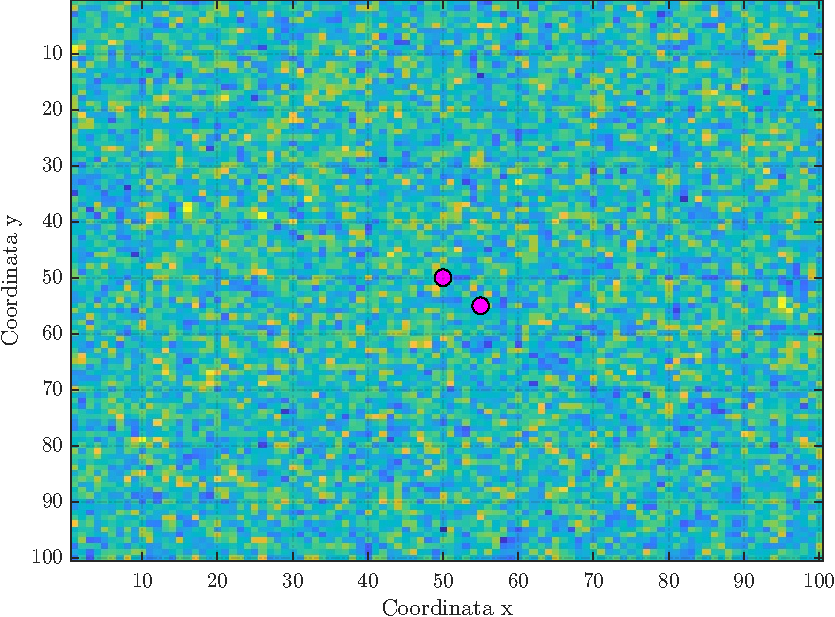
\includegraphics[height=152px]{Immagini/1. Modello base/Sim. proc. gaussiano, theta = 0.5}}\quad
	\subfigure[]{\label{}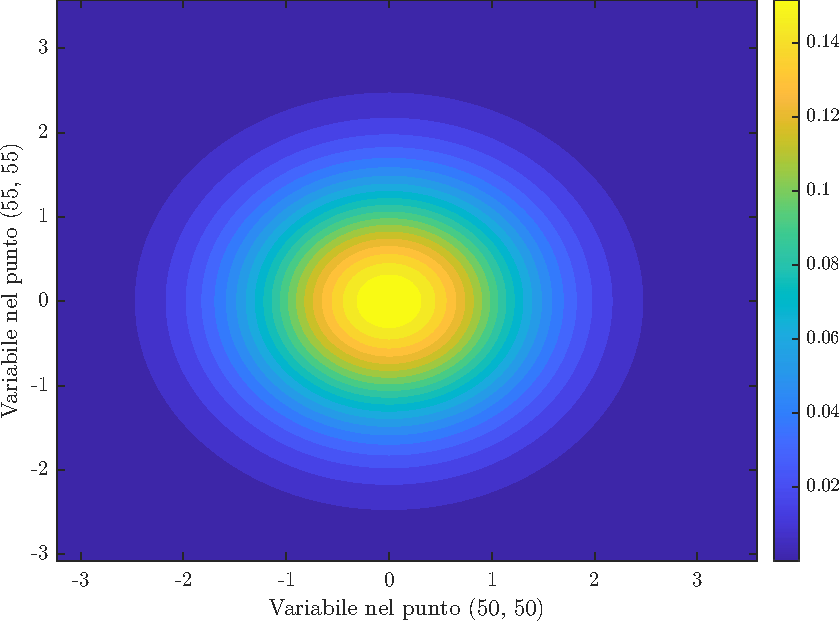
\includegraphics[height=152px]{Immagini/1. Modello base/Sim. var. casuali, theta = 0.5}}\quad
	\subfigure[]{\label{}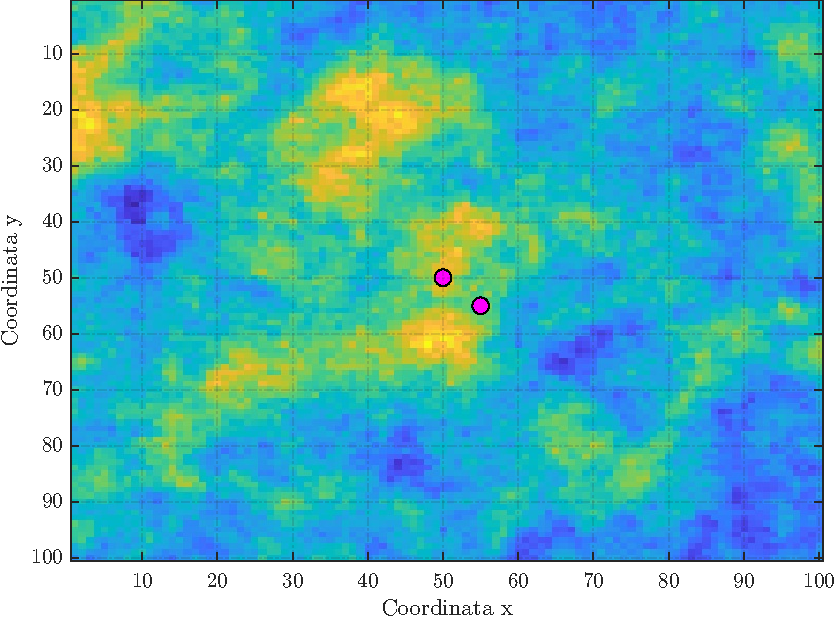
\includegraphics[height=152px]{Immagini/1. Modello base/Sim. proc. gaussiano, theta = 10}}\quad
	\subfigure[]{\label{}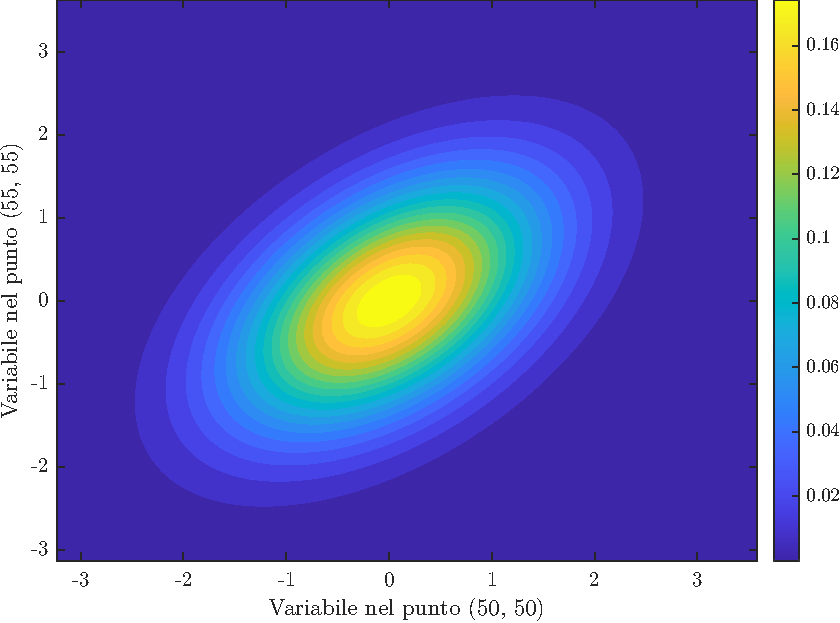
\includegraphics[height=152px]{Immagini/1. Modello base/Sim. var. casuali, theta = 10}}\quad
	\subfigure[]{\label{}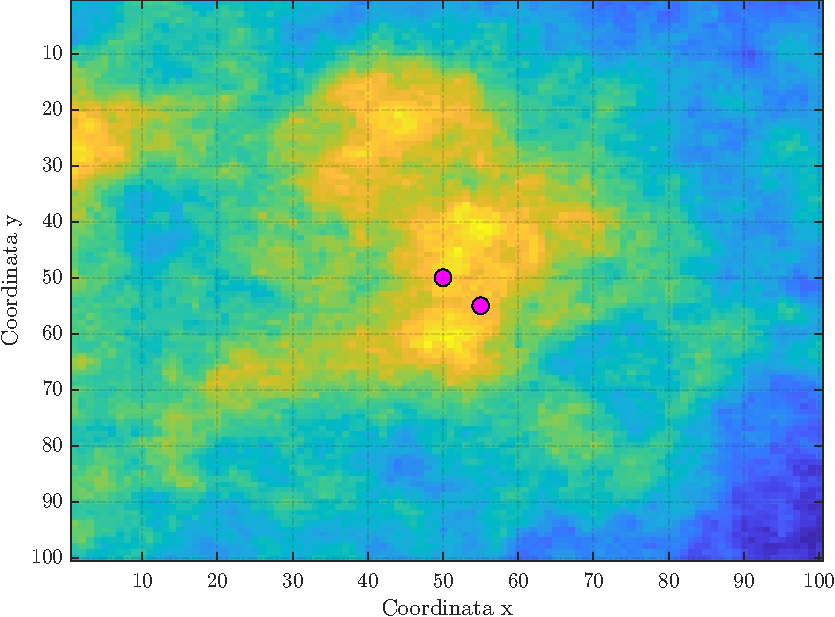
\includegraphics[height=152px]{Immagini/1. Modello base/Sim. proc. gaussiano, theta = 100}}\quad
	\subfigure[]{\label{}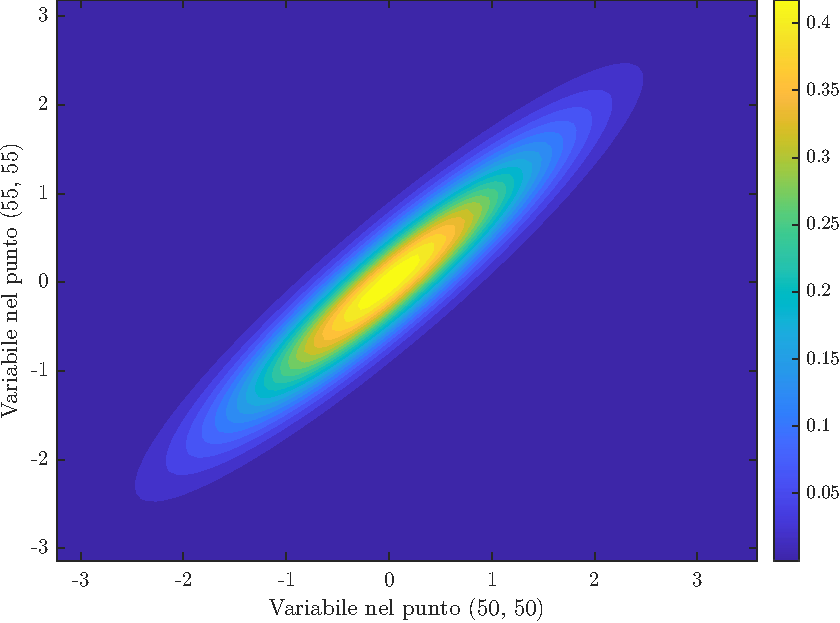
\includegraphics[height=152px]{Immagini/1. Modello base/Sim. var. casuali, theta = 100}}
	\caption[Simulazione di un processo spaziale gaussiano su un piano cartesiano al variare di $\theta$]{simulazione di un processo spaziale gaussiano su un piano cartesiano regolare e rispettiva densità di probabilità congiunta della normale bi-variata riferita ai punti $(50, 50)$ e $(55, 55)$ con $\theta=0.5$ (a, b), \num{10} (c, d) e \num{100} (e, f).}
	\label{sim_proc_gaussiano}
\end{figure}

\subsection[Parametri da stimare]{Parametri da stimare}
In conclusione, viene riportato il vettore $\boldsymbol{\psi}\in\mathbb{R}^{(n_\epsilon + n_\beta\cdot b + 3\cdot n_z)\times 1}$ contenente i parametri da stimare:
\begin{equation}
	\boldsymbol{\psi} = (\mathbf{c}_\epsilon^\top, \mathbf{c}_\beta^\top, \mathbf{g}^\top, \mathbf{v}^\top, \boldsymbol{\theta}^\top)^\top.
\end{equation}
Alcuni di essi possono essere calcolati in forma chiusa, altri richiedono l'ottimizzazione numerica.
\par Inoltre, è necessario ricostruire la componente latente, operazione complessa che può essere eseguita integrando il filtro di Kalman (e smoother) nel passo E dell'algoritmo EM.

\section[Cenni sull'algoritmo EM]{Cenni sull'algoritmo EM}
L'algoritmo EM (Expectation-Maximization) è una tecnica di ottimizzazione iterativa per determinare la stima a massima verosimiglianza (Maximum Likelihood Estimate, o MLE) \textbf{in presenza di dati mancanti o nascosti (variabili latenti)}. Nella stima ML si desidera determinare i parametri del modello per i quali i dati osservati risultano essere i più verosimili~\cite{paper_EM_algorithm}. \par Ogni iterazione dell'algoritmo EM consiste in due passi:
\begin{itemize}
	\item \textbf{passo E}: a partire dalla stima corrente dei parametri $\boldsymbol{\theta}_n$ e dai dati disponibili $\mathbf{x}$, quelli mancanti e/o nascosti vengono prima stimati e poi impiegati per determinare l'\textit{aspettativa condizionale} $Q(\boldsymbol{\theta},\boldsymbol{\theta}_n)$, una semplificazione della stima corrente della funzione di verosimiglianza $l(\boldsymbol{\theta}|\boldsymbol{\theta}_n)$;
	\item \textbf{passo M}: $Q(\boldsymbol{\theta},\boldsymbol{\theta}_n)$ viene ottimizzata per determinare $\boldsymbol{\theta}_{n+1}$, assumendo che i dati mancanti siano noti. Le stime di questi, ottenute precedentemente nel passo E, sono utilizzate al posto dei dati mancanti effettivi.
\end{itemize}
La convergenza dell'algoritmo è garantita dall'aumento della verosimiglianza a ogni iterazione.

\subsection{Derivazione del passo E}
Sia $\mathbf{x}$ un vettore di dati aleatori appartenenti a una famiglia di modelli parametrizzata. Si desidera trovare il valore delle incognite $\boldsymbol{\theta}$ tale che la verosimiglianza $L(\boldsymbol{\theta})=P(\mathbf{x} | \boldsymbol{\theta})$ sia massima. L'algoritmo EM garantisce che $L(\boldsymbol{\theta}) > L(\boldsymbol{\theta}_n)$; applicando il logaritmo naturale\footnote{semplificazione che spesse volte viene adottata per trasformare il prodotto di densità di probabilità che caratterizza $L$ (assumendo l'indipendenza tra i campioni) in una somma.} si ottiene:
\begin{equation}
	\ln(P(\mathbf{x}|\boldsymbol{\theta}) - P(\mathbf{x}|\boldsymbol{\theta}_n)) > 0.
	\label{eq_dis_verosimiglianza}
\end{equation}
Tale risultato deriva dal fatto che $L(\boldsymbol{\theta})$ si può dimostrare essere strettamente positiva. Tuttavia, i dati osservati $\mathbf{x}$ non dipendono soltanto dai parametri da stimare, ma anche dai valori assunti dalle componenti latenti $\mathbf{z}$ (da ricostruire utilizzando il filtro di Kalman). Infatti, la probabilità totale $P(\mathbf{x}|\boldsymbol{\theta})$ può essere riscritta in termini di $\mathbf{z}$ come:
\[
	P(\mathbf{x}|\boldsymbol{\theta}) = \sum_{\mathbf{z}}^{}P(\mathbf{x}|\boldsymbol{\theta}, \mathbf{z})\cdot P(\mathbf{z}|\boldsymbol{\theta}).
\]
Di conseguenza, l'equazione \ref{eq_dis_verosimiglianza} diventa:
\begin{equation}
	L(\boldsymbol{\theta}) - L(\boldsymbol{\theta}_n) = \ln\sum_{\mathbf{z}}^{} P(\mathbf{x}|\boldsymbol{\theta}, \mathbf{z})\cdot P(\mathbf{z}|\boldsymbol{\theta}) - \ln P(\mathbf{x}|\boldsymbol{\theta}_n).
	\label{eq_dis_verosimiglianza_completa}
\end{equation}
A partire dall'introduzione del termine \textcolor{orange}{$P(\mathbf{z}|\mathbf{x},\boldsymbol{\theta}_n)$} nell'equazione \ref{eq_dis_verosimiglianza_completa}, è possibile eseguire la seguente derivazione:
\begin{equation}
	\begin{split}
		L(\boldsymbol{\theta}) - L(\boldsymbol{\theta}_n) & = -\ln P(\mathbf{x}|\boldsymbol{\theta}_n) + \ln\sum_{\mathbf{z}}^{} P(\mathbf{x}|\mathbf{z},\boldsymbol{\theta})\cdot P(\mathbf{z}|\boldsymbol{\theta})\cdot\frac{\textcolor{orange}{P(\mathbf{z}|\mathbf{x},\boldsymbol{\theta}_n)}}{\textcolor{orange}{P(\mathbf{z}|\mathbf{x},\boldsymbol{\theta}_n)}} \\
		& = \textcolor{blue}{-\ln P(\mathbf{x}|\boldsymbol{\theta}_n)} + \ln\sum_{\mathbf{z}}^{} \textcolor{orange}{P(\mathbf{z}|\mathbf{x},\boldsymbol{\theta}_n)}\cdot\frac{P(\mathbf{x}|\mathbf{z},\boldsymbol{\theta})\cdot P(\mathbf{z}|\boldsymbol{\theta})}{\textcolor{orange}{P(\mathbf{z}|\mathbf{x},\boldsymbol{\theta}_n)}} \\
		& = \ln\sum_{\mathbf{z}}^{} \textcolor{orange}{P(\mathbf{z}|\mathbf{x},\boldsymbol{\theta}_n)}\cdot\frac{P(\mathbf{x}|\mathbf{z},\boldsymbol{\theta})\cdot P(\mathbf{z}|\boldsymbol{\theta})}{\textcolor{orange}{P(\mathbf{z}|\mathbf{x},\boldsymbol{\theta}_n)}\cdot\textcolor{blue}{ P(\mathbf{x}|\boldsymbol{\theta}_n)}} \\
		& \geq\sum_{\mathbf{z}}^{}\textcolor{orange}{P(\mathbf{z}|\mathbf{x},\boldsymbol{\theta}_n)}\cdot\ln\frac{P(\mathbf{x}|\mathbf{z},\boldsymbol{\theta})\cdot P(\mathbf{z}|\boldsymbol{\theta})}{\textcolor{orange}{P(\mathbf{z}|\mathbf{x},\boldsymbol{\theta}_n)}\cdot P(\mathbf{x}|\boldsymbol{\theta}_n)} \triangleq\Delta(\boldsymbol{\theta}|\boldsymbol{\theta}_n);
	\end{split}
\end{equation}
per il corollario della disuguaglianza di Jensen\footnote{sia $f$ una funzione concava ($\ln$ lo è) e $\lambda_1,\dots\lambda_n\in [0,1]$ tali che $\sum_{i=1}^{n}\lambda_i = 1$, allora $f(\sum_{i=1}^{n}\lambda_i\cdot x_i)\geq\sum_{i=1}^{n}\lambda_i\cdot f(x_i)$. Il teorema è applicabile perché $\sum_{\mathbf{z}}^{} P(\mathbf{z}|\mathbf{x},\boldsymbol{\theta}_n)=1$.}. Pertanto:
\begin{equation}
	L(\boldsymbol{\theta})\geq L(\boldsymbol{\theta}_n)+\Delta(\boldsymbol{\theta}|\boldsymbol{\theta}_n)\triangleq l(\boldsymbol{\theta}|\boldsymbol{\theta}_n).
\end{equation}
La figura \ref{grafico_verosimiglianza} materializza il risultato appena ottenuto: l'approssimazione di $L(\boldsymbol{\theta})$ in un intorno di $\boldsymbol{\theta}_n$ non sovrastima la vera funzione di verosimiglianza, quindi ottimizzare l'approssimazione comporta la massimizzazione implicita anche di $L(\boldsymbol{\theta})$. Si ricorda, inoltre, che $\boldsymbol{\theta}_n = \text{arg}\,\max\limits_{\boldsymbol{\theta}} \ l(\boldsymbol{\theta}|\boldsymbol{\theta}_{n-1})$.

\begin{figure}[htp]
	\centering
	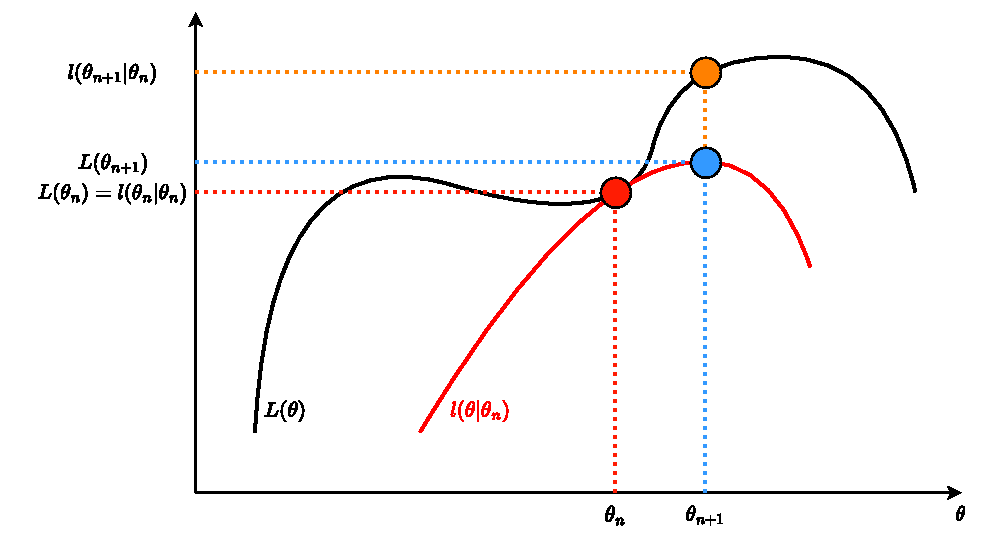
\includegraphics[height=180px]{Immagini/1. Modello base/Grafico verosimiglianza}
	\caption[Confronto tra la vera funzione di verosimiglianza $L(\theta)$ e la sua approssimazione in $\theta_n$.]{confronto tra la vera funzione di verosimiglianza $L(\theta)$ e la sua approssimazione in un intorno di $\theta_n$. Da notare che lo stimatore $l(\theta |\theta_n)$ non sovrastima la funzione reale.}
	\label{grafico_verosimiglianza}
\end{figure}

\subsection{Derivazione del passo M}
Dopo aver stimato nel passo E l'approssimazione $l(\boldsymbol{\theta}|\boldsymbol{\theta}_n)$  della vera funzione di verosimiglianza $L(\boldsymbol{\theta})$, è necessario ottimizzarla per determinare $\boldsymbol{\theta}_{n+1}$. Nello specifico:
\begin{equation}
	\begin{split}
		\boldsymbol{\theta}_{n+1} & = \text{arg}\,\max\limits_{\boldsymbol{\theta}}\  l(\boldsymbol{\theta}|\boldsymbol{\theta}_n) \\
		& =  \text{arg}\,\max\limits_{\boldsymbol{\theta}}\left\{ \textcolor{orange}{L(\boldsymbol{\theta}_n)} + \sum_{\mathbf{z}}^{} P(\mathbf{z}|\mathbf{x},\boldsymbol{\theta}_n)\cdot\ln\frac{P(\mathbf{x}|\mathbf{z},\boldsymbol{\theta})\cdot P(\mathbf{z}|\boldsymbol{\theta})}{\textcolor{orange}{P(\mathbf{z}|\mathbf{x},\boldsymbol{\theta}_n)}\cdot\textcolor{orange}{P(\mathbf{x}|\boldsymbol{\theta}_n)}}\right\} \\
		& = \text{arg}\,\max\limits_{\boldsymbol{\theta}}\left\{\sum_{\mathbf{z}}^{} P(\mathbf{z}|\mathbf{x},\boldsymbol{\theta}_n)\cdot\ln\textcolor{blue}{ P(\mathbf{x}|\mathbf{z},\boldsymbol{\theta})\cdot P(\mathbf{z}|\boldsymbol{\theta})}\right\}\\
		& = \text{arg}\,\max\limits_{\boldsymbol{\theta}}\left\{\sum_{\mathbf{z}}^{}P(\mathbf{z}|\mathbf{x},\boldsymbol{\theta}_n)\cdot\ln \textcolor{blue}{P(\mathbf{x},\mathbf{z}|\boldsymbol{\theta})}\right\}\\
		& = \text{arg}\,\max\limits_{\boldsymbol{\theta}}\left\{\text{E}_{\mathbf{z}|\mathbf{x},\boldsymbol{\theta}_n}\ln P(\mathbf{x},\mathbf{z}|\boldsymbol{\theta})\right\}\\
		& = \text{arg}\,\max\limits_{\boldsymbol{\theta}}\ Q(\boldsymbol{\theta},\boldsymbol{\theta}_n).
	\end{split}
\label{eq_derivazione_step_M}
\end{equation}
I termini in arancione vengono rimossi poiché costanti rispetto a $\boldsymbol{\theta}$, quindi non influenzano la ricerca dell'ottimo, mentre a quelli blu viene applicato il teorema di Bayes. \par Attraverso la riscrittura di $l(\boldsymbol{\theta}|\boldsymbol{\theta}_n)$ in $Q(\boldsymbol{\theta},\boldsymbol{\theta}_n)$ mediante la derivazione \ref{eq_derivazione_step_M}, si può comprendere l'idea che sta alla base dell'algoritmo EM: la log-verosimiglianza viene iterativamente corretta tramite la stima corrente della densità di probabilità delle variabili latenti $\mathbf{z}$, un'approssimazione ottenuta nel passo E a partire dai dati osservati $\mathbf{x}$ e dalla stima corrente dei coefficienti $\boldsymbol{\theta}_n$.

	\chapter[Il concetto di geo-potenziale e il nuovo modello]{Il concetto di geo-potenziale e descrizione del nuovo modello}
	\chapter[Stima EM del modello fp-HDGM]{Stima EM del modello fp-HDGM}

Dopo aver presentato nel capitolo precedente il modello fp-HDGM, in questo vengono illustrate le formule di stima. Innanzitutto viene derivata la funzione di verosimiglianza $L(\boldsymbol{\theta})$, poi la componente $\Omega(t)$ del valore atteso condizionato $Q(\boldsymbol{\theta}, \boldsymbol{\theta}_n)$; essa è l'oggetto dell'ottimizzazione svolta nel passo M per stimare il nuovo parametro $\rho$. Per la nomenclatura si rimanda alla sezione \ref{equazioni_modello_base}.

\section[La funzione di verosimiglianza]{La funzione di verosimiglianza}
La stima dei parametri $\boldsymbol{\theta}$ e dalla variabile latente spazio-temporale $\mathbf{z}(\mathbf{s}, t)$ è basata sull'approccio a massima verosimiglianza~\citep{paper_f_HDGM}.

\subsection[Rappresentazione matriciale del modello fp-HDGM]{Rappresentazione matriciale del modello fp-HDGM}
Si misuri la variabile $y(\mathbf{s}_i, l_j, t)$ per ogni valore $l_j\in \mathcal{L}$\footnote{per semplicità di notazione, si assume l'assenza di dati mancanti, ovvero $q$ osservazioni per ogni $\mathbf{s}_i$ e $t$.} in uno specifico punto nello spazio $\mathbf{s}_i\in\mathcal{S} = \{(s_{lon,1}, s_{lat,1}),\dots,(s_{lon,n}, s_{lat,n})\}$ e istante temporale $t$. Il vettore risultante è:
\[
\mathbf{y}(\mathbf{s}_i, t) = \left[ y(\mathbf{s}_i, l_1, t) \ \dots \ y(\mathbf{s}_i, l_j, t) \ \dots \ y(\mathbf{s}_i, l_q, t) \right]^\top_{q\times 1}.
\]
Esso prende il nome di \textit{profilo} osservato. Se si percorrono tutti i punti di misura $\mathcal{S}$, allora si costruisce la seguente matrice:
\[
\mathbf{y}_t = \left[ {y}(\mathbf{s}_1, t) \ \dots \ {y}(\mathbf{s}_k, t) \ \dots \ {y}(\mathbf{s}_n, t) \right]^\top_{N\times 1};
\]
dove $N=n\cdot q$. Applicando le equazioni alla struttura dati appena definita, si ottiene la seguente rappresentazione matriciale del modello fp-HDGM:
\begin{equation}
	\mathbf{y}_t = H\cdot\boldsymbol{\omega}_t;
	\label{eq_matriciale_y_fp_HDGM}
\end{equation}
\begin{equation}
	\boldsymbol{\omega}_t = \boldsymbol{\mu}_t + \boldsymbol{\epsilon}_t
\end{equation}
\begin{equation}
	\boldsymbol{\mu}_t = \mathbf{X}_t\cdot\Phi_{\beta, t}\cdot\mathbf{c}_\beta + \Phi_{z, t}\cdot\mathbf{z}_t;
\end{equation}
\begin{equation}
	\mathbf{z}_t = \tilde{G}\cdot\mathbf{z}_{t-1} + \boldsymbol{\eta}_t.
	\label{eq_matriciale_z_fp_HDGM}
\end{equation}
$H\in\mathbb{R}^{N\times 1}$ è una matrice diagonale contenente i coefficienti $h_i = \left( 1 + \sum_{\mathbf{s}\in\mathcal{S}/\mathbf{s}_i}^{\mathcal{S}} e^{\frac{\|\mathbf{s} - \mathbf{s}_i\|}{\rho}}\right)^{-1}$ ripetuti $q$ volte per ogni punto di misura, $X_t\in\mathbb{R}^{N\times b}$ è la matrice delle covariate, $\boldsymbol{\Phi}_{\beta, t}\in\mathbb{R}^{b\times (b\cdot n_\beta)}$ e $\boldsymbol{\Phi}_{z, t}\in\mathbb{R}^{N\times(n\cdot n_z)}$ contengono i valori delle basi rispettivamente per $\boldsymbol{\beta}$ e per $\mathbf{z}$, mentre $\tilde{G}\in\mathbb{R}^{(n\cdot n_z)\times (n\cdot n_z)}$ è una matrice diagonale a blocchi costruita con $G$, ossia la matrice di transizione. Infine, $\boldsymbol{\epsilon}_t\in\mathbb{R}^{N}$ ed $\boldsymbol{\eta}_t\in\mathbb{R}^{n\cdot n_z}$ sono i vettori delle variabili casuali: il primo descrive il rumore sull'uscita, il secondo la correlazione spaziale.

\subsection[Distribuzioni delle variabili casuali]{Distribuzioni delle variabili casuali}
Pre-moltiplicando per $H^{-1}$ ambo i termini dell'equazione~\ref{eq_matriciale_y_fp_HDGM}, si ottiene:
\[
H^{-1}\cdot\mathbf{y}_t  = \boldsymbol{\mu}_t + \boldsymbol{\epsilon}_t.
\]
$\boldsymbol{\epsilon}_t$ è un vettore di variabili aleatorie distribuite normalmente con media $\boldsymbol{\mu}_\epsilon\in\mathbb{R}^{N}$ nulla e varianza $\Sigma_\epsilon\in\mathbb{R}^{N\times N}$, una matrice diagonale costruita utilizzando $\sigma_\epsilon(l)$, ossia la varianza funzionale. Di conseguenza:
\[
H^{-1}\cdot\mathbf{y}_t\backsim\mathcal{N}_N\left\{\boldsymbol{\mu}_t, \Sigma_\epsilon\right\}.
\]
Un discorso simile si può fare per l'equazione~\ref{eq_matriciale_z_fp_HDGM}; $\boldsymbol{\eta}_t$ è anch'esso un vettore di variabili casuali distribuite normalmente con media $\boldsymbol{\mu}_\eta\in\mathbb{R}^{n\cdot n_z}$ nulla, tuttavia la sua matrice di varianze e covarianze $\Sigma_\eta\in\mathbb{R}^{(n\cdot n_z)\times(n\cdot n_z)}$ è diagonale a blocchi, costruita utilizzando $\Gamma_\eta\in\mathbb{R}^{n\times n}$, ovvero la matrice di correlazione spaziale. Pertanto:
\[
\mathbf{z}_t\backsim\mathcal{N}_{n\cdot n_z}\left\{\tilde{G}\cdot\mathbf{z}_{t-1}, \Gamma_\eta\right\}.
\]

\subsection[Derivazione della funzione di verosimiglianza]{Derivazione della funzione di verosimiglianza}
Siano $X$, $Y$ e $Z$ le matrici contenenti rispettivamente i valori assunti dalle covariate, dall'uscita e dalle componenti latenti. Per definizione, la funzione di verosimiglianza ha la seguente espressione:
\begin{equation}
	L(\boldsymbol{\theta}; Y,Z,X) = L(\boldsymbol{\theta}; X)\cdot L(\boldsymbol{\theta}; Z|X)\cdot L(\boldsymbol{\theta}; Y|Z,X).
	\label{eq_gen_verosimiglianza}
\end{equation}
La quantità $L(\boldsymbol{\theta}; X)$ è unitaria perché le covariate sono deterministiche, mentre $L(\boldsymbol{\theta}; Z|X) = L(\boldsymbol{\theta}; Z)$ poiché $X$ e $Z$ sono indipendenti tra loro. Quindi, l'equazione~\ref{eq_gen_verosimiglianza} diventa:
\begin{equation}
	L(\boldsymbol{\theta}; Y,Z,X) =  L(\boldsymbol{\theta}; Z)\cdot L(\boldsymbol{\theta}; Y|Z,X).
	\label{eq_gen_verosimiglianza_2}
\end{equation}
Nello specifico:
\begin{equation}
	\begin{split}
		L(\boldsymbol{\theta}; Y|Z, X) & = \prod_{t=1}^{T}\left(|\Sigma_\epsilon|^\frac{1}{2}\cdot\left(2\pi\right)^\frac{n\cdot q}{2}\right)^{-1}\cdot e^{-\frac{1}{2}\left(H^{-1}\mathbf{y}_t - \boldsymbol{\mu}_t\right)^\top\Sigma_\epsilon^{-1}\left(H^{-1}\mathbf{y}_t - \boldsymbol{\mu}_t\right)} \\
		& = \left(|\Sigma_\epsilon|^\frac{1}{2}\cdot\left(2\pi\right)^\frac{n\cdot q}{2}\right)^{-T}\cdot\prod_{t=1}^{T} e^{-\frac{1}{2}\left(H^{-1}\mathbf{y}_t - \boldsymbol{\mu}_t\right)^\top\Sigma_\epsilon^{-1}\left(H^{-1}\mathbf{y}_t - \boldsymbol{\mu}_t\right)};
	\end{split}
\end{equation}
e
\begin{equation}
	\begin{split}
		L(\boldsymbol{\theta}; Z) & = L(\boldsymbol{\theta}; \mathbf{z}_0)\cdot L(\boldsymbol{\theta}; \mathbf{z}_1|\mathbf{z}_0)\cdots L(\boldsymbol{\theta}; \mathbf{z}_T|\mathbf{z}_0, \mathbf{z}_1,\dots\mathbf{z}_{T-1}) \\
		& = L(\boldsymbol{\theta}; \mathbf{z}_0)\cdot L(\boldsymbol{\theta}; \mathbf{z}_1|\mathbf{z}_0)\cdots L(\boldsymbol{\theta}; \mathbf{z}_T|\mathbf{z}_{T-1})\\
		& = L(\boldsymbol{\theta}; \mathbf{z}_0)\cdot\prod_{t=1}^{T}L(\boldsymbol{\theta};\mathbf{z}_t|\mathbf{z}_{t-1});
	\end{split}
	\label{eq_verosimiglianza_y}
\end{equation}
poiché l'autocorrelazione del processo gaussiano markoviano è a un passo ($\tau = 1$). Da segnalare, inoltre, che l'operatore $|\cdot|$ indica il determinante. Aumentando il livello di dettaglio si ottiene:
\begin{equation}
	L(\boldsymbol{\theta}; \mathbf{z}_0) = \left(|\Sigma_0|^\frac{1}{2}\cdot\left(2\pi\right)^\frac{n\cdot n_z}{2}\right)^{-1}\cdot e^{-\frac{1}{2}\left(\mathbf{z}_0 - \boldsymbol{\mu}_0 \right)^\top\Sigma_0^{-1}\left(\mathbf{z}_0 - \boldsymbol{\mu}_0 \right)};
\end{equation}
e
\begin{equation}
	\begin{split}
		\prod_{t=1}^{T}L(\boldsymbol{\theta};\mathbf{z}_t|\mathbf{z}_{t-1}) & = \prod_{t=1}^{T}\left(|\Sigma_\eta|^\frac{1}{2}\cdot\left(2\pi\right)^\frac{n\cdot n_z}{2}\right)^{-1}\cdot e^{-\frac{1}{2}\left(\mathbf{z}_t - \tilde{G}\boldsymbol{z}_{t-1} \right)^\top\Sigma_\eta^{-1}\left(\mathbf{z}_t - \tilde{G}\boldsymbol{z}_{t-1} \right)}\\
		& = \left(|\Sigma_\eta|^\frac{1}{2}\cdot\left(2\pi\right)^\frac{n\cdot n_z}{2}\right)^{-T}\cdot\prod_{t=1}^{T}e^{-\frac{1}{2}\left(\mathbf{z}_t - \tilde{G}\boldsymbol{z}_{t-1} \right)^\top\Sigma_\eta^{-1}\left(\mathbf{z}_t - \tilde{G}\boldsymbol{z}_{t-1} \right)}.
	\end{split}
\end{equation}
Per rimuovere i prodotti e per predisporre la funzione di verosimiglianza alla minimizzazione, all'equazione~\ref{eq_gen_verosimiglianza_2} viene applicato il logaritmo naturale negato, ossia:
\begin{equation}
	-2\ln L(\boldsymbol{\theta}; Y, Z, X) = -2\ln L(\boldsymbol{\theta}; Z) - 2\ln L(\boldsymbol{\theta}; Y|Z,X);
\end{equation}
con:
\begin{equation}
	\begin{split}
		- 2\ln L(\boldsymbol{\theta}; Y|Z,X) & = T\ln|\Sigma_\epsilon| +\sum_{t=1}^{T}+\left(H^{-1}\mathbf{y}_t - \boldsymbol{\mu}_t\right)^\top\Sigma_\epsilon^{-1}\left(H^{-1}\mathbf{y}_t - \boldsymbol{\mu}_t\right);
	\end{split}
\end{equation}
\begin{equation}
	\begin{split}
		- 2\ln L(\boldsymbol{\theta}; \mathbf{z}_0) & = T\ln|\Sigma_0| + \left(\mathbf{z}_0 - \boldsymbol{\mu}_0 \right)^\top\Sigma_0^{-1}\left(\mathbf{z}_0 - \boldsymbol{\mu}_0 \right);
	\end{split}
\end{equation}
e
\begin{equation}
	\begin{split}
		- 2\ln\prod_{t=1}^{T} L(\boldsymbol{\theta}; \mathbf{z}_t|\mathbf{z}_{t-1}) & = T\ln|\Sigma_\eta| +\sum_{t=1}^{T} \left(\mathbf{z}_t - \tilde{G}\mathbf{z}_{t-1} \right)^\top\Sigma_\eta^{-1}\left(\mathbf{z}_t - \tilde{G}\mathbf{z}_{t-1} \right).
	\end{split}
\end{equation}
I termini $T(n\cdot q)\ln 2\pi$, $(n\cdot n_z)\ln 2\pi$ e $T(n\cdot n_z)\ln 2\pi$ sono stati rimossi poiché sono costanti, quindi non influenzano la ricerca di $\hat{\boldsymbol{\theta}}=\text{arg}\,\min\limits_{\boldsymbol{\theta}} -2\ln L(\boldsymbol{\theta}; Y, Z, X)$. \par Riassumendo ed esplicitando i singoli termini di $\boldsymbol{\theta}$, si ottiene:
\begin{equation}
	\begin{split}
		-2\ln L(\boldsymbol{\theta}; Y, Z, X) & =  T\ln|\Sigma_\epsilon\left(\textcolor{black}{\mathbf{c}_\epsilon}\right)| \\
		& + \sum_{t=1}^{T} \left(H^{-1}(\textcolor{black}{\rho})\cdot\mathbf{y}_t - \boldsymbol{\mu}_t(\textcolor{black}{\mathbf{c}_\beta})\right)^\top\Sigma_\epsilon^{-1}\left(H^{-1}(\textcolor{black}{\rho})\cdot\mathbf{y}_t - \boldsymbol{\mu}_t(\textcolor{black}{\mathbf{c}_\beta})\right) \\
		& + \ln|\Sigma_0| \\
		& + (\mathbf{z}_0 - \boldsymbol{\mu}_0)^\top\Sigma_0^{-1}(\mathbf{z}_0 - \boldsymbol{\mu}_0) \\
		& + T\ln |\Sigma_\eta(\textcolor{black}{\mathbf{v},\boldsymbol{\lambda}})| \\
		& + \sum_{t=1}^{T}\left(\mathbf{z_t}-\tilde{G}(\textcolor{black}{\mathbf{g}})\cdot\mathbf{z}_{t-1}\right)^\top\Sigma_\eta^{-1}(\textcolor{black}{\mathbf{v},\boldsymbol{\lambda}})\left(\mathbf{z_t}-\tilde{G}(\textcolor{black}{\mathbf{g}})\cdot\mathbf{z}_{t-1}\right).
	\end{split}
	\label{eq_fin_verosimiglianza}
\end{equation}
Il secondo addendo è quello che dev'essere minimizzato per determinare $\rho$.

\section[Il valore atteso condizionato]{Il valore atteso condizionato}
Il valore atteso condizionato $Q(\boldsymbol{\theta}, \boldsymbol{\theta}_n)$ è l'oggetto della massimizzazione\footnote{minimizzazione se viene applicato il logaritmo naturale negato alla funzione di verosimiglianza.} compiuta dal passo M per determinare $\boldsymbol{\theta}_n$, ossia la stima all'iterazione $n$ dei parametri da identificare. Il ricorso all'algoritmo EM è necessario poiché nel modello compaiono delle variabili latenti $\mathbf{z}$ che devono essere ricostruite, di conseguenza non si può minimizzare direttamente la funzione~\ref{eq_fin_verosimiglianza}.

\subsection[Derivazione di Q$(\boldsymbol{\theta}, \boldsymbol{\theta}_n)$]{Derivazione di Q$(\boldsymbol{\theta}, \boldsymbol{\theta}_n)$}
L'espressione del valore atteso condizionato è la seguente~\citep{paper_GRASPA}:
\begin{equation}
	\begin{split}
		Q(\boldsymbol{\theta},\boldsymbol{\theta}_n) & = \text{E}_{\boldsymbol{\theta}_n}\left\{T\ln|\Sigma_0| + \text{tr}\left(\Sigma_0^{-1}\left(\mathbf{z}_0 - \boldsymbol{\mu}_0\right)\left(\mathbf{z}_0 - \boldsymbol{\mu}_0\right)^\top\right)\bigg| Y^{(1)}\right\} \\
		& + \text{E}_{\boldsymbol{\theta}_n}\left\{T\ln|\Sigma_\eta| + \text{tr}\left(\Sigma_\eta^{-1}\sum_{t=1}^{T}\left(\mathbf{z}_t - \tilde{G}\mathbf{z}_{t-1}\right)\left(\mathbf{z}_t - \tilde{G}\mathbf{z}_{t-1}\right)^\top\right)\bigg| Y^{(1)}\right\} \\
		& + \text{E}_{\boldsymbol{\theta}_n}\left\{T\ln|\Sigma_\epsilon| + \text{tr}\left(\Sigma_\epsilon^{-1}\sum_{t=1}^{T}\mathbf{e}_t\cdot\mathbf{e}_t^\top\right)\bigg| Y^{(1)}\right\};
	\end{split}
	\label{eq_Q}
\end{equation}
dove $\mathbf{e}_t = H^{-1}(\rho)\cdot\mathbf{y}_t - \boldsymbol{\mu}_t$ e $Y^{(1)}$ rappresenta le osservazioni disponibili\footnote{si ricorda che l'algoritmo EM è in grado stimare $\mathbf{y}_t$ nei punti e negli istanti in cui essa è ignota.}. Il terzo addendo dell'equazione~\ref{eq_Q} viene rinominato in $m(\rho)$; nello specifico:
\begin{equation}
	\begin{split}
		m(\rho) & = \text{E}_{\boldsymbol{\theta}_n}\left\{T\ln|\Sigma_\epsilon| \ \bigg|Y^{(1)}\right\} + \text{E}_{\boldsymbol{\theta}_n}\left\{\text{tr}\left(\Sigma_\epsilon^{-1}\sum_{t=1}^{T}\mathbf{e}_t\cdot\mathbf{e}_t^\top\right)\bigg|Y^{(1)}\right\} \\
		& = T\ln|\Sigma_\epsilon| + \text{tr}\left(\text{E}_{\boldsymbol{\theta}_n}\left\{\Sigma_\epsilon^{-1}\sum_{t=1}^{T}\mathbf{e}_t\cdot\mathbf{e}_t^\top \ \bigg|Y^{(1)}\right\}\right) \\
		& = T\ln|\Sigma_\epsilon| + \text{tr}\left(\Sigma_\epsilon^{-1}\sum_{t=1}^{T}E_{\boldsymbol{\theta}_n}\left\{\mathbf{e}_t\cdot\mathbf{e}_t^\top \ \bigg| Y^{(1)}\right\}\right).
	\end{split}
\label{eq_f_rho}
\end{equation}
La quantità $m(\rho)$ del valore atteso condizionato $Q(\boldsymbol{\theta}, \boldsymbol{\theta}_n)$ è l'unica che dipende da $\rho$, l'unica che dev'essere ottimizzata per stimare il nuovo parametro.

\subsection[Espressione della matrice $\Omega_t$]{Espressione della matrice $\Omega_t$}
Sia $\text{E}_{\boldsymbol{\theta}_n}\left\{\mathbf{e}_t\cdot\mathbf{e}_t^\top \ \bigg|Y^{(1)}\right\} = \Omega_t\in\mathbb{R}^{(n\cdot q)\times(n\cdot q)}$, allora~\citep{paper_TS_book}:
\begin{equation}
	\begin{split}
		\Omega_t & = \begin{bmatrix}
			H^{(1)^{-1}}\cdot\mathbf{y}_t^{(1)} - X_t^{(1)}\cdot\Phi_{\beta, t}\cdot\mathbf{c}_\beta - \Phi_{z, t}\cdot\mathbf{z}_t \\
			R_{21, t}\cdot R_{11,t}^{-1}\cdot\mathbf{e}_t^{(1)}
		\end{bmatrix}_{(n\times q)\times 1} \cdot \begin{bmatrix}
		\mathbf{e}_t \\
		R_{21,t}\cdot R_{11, t}^{-1}\cdot\mathbf{e}_t^{(1)}
	\end{bmatrix}^\top_{(n\times q)\times 1} \\
	& + \begin{bmatrix}
		\Phi_{z,t}^{(1)} \\
		R_{21, t}\cdot R_{11, t}^{-1}\cdot\Phi_{z,t}^{(1)}
	\end{bmatrix}_{(n\cdot q)\times(n\cdot n_z)}\cdot\Sigma_{\eta, t}^{(1)}\cdot \begin{bmatrix}
		\Phi_{z,t}^{(1)} \\
	R_{21, t}\cdot R_{11, t}^{-1}\cdot\Phi_{z,t}^{(1)}
	\end{bmatrix}^\top_{(n\cdot n_z)\times(n\cdot q)} \\
	& + \begin{bmatrix}
		\mathbf{0} & \mathbf{0}\\
		\mathbf{0} & R_{22,t} - R_{21,t}\cdot R_{11,t}^{-1}\cdot R_{11, t}
	\end{bmatrix}_{(n\cdot q)\times(n\cdot q)}.
	\end{split}
	\label{eq_omega_1}
\end{equation}
\[
	R_t = \Sigma_{\epsilon, t} = \begin{bmatrix}
		R_{11, t} & R_{12, t} \\ R_{21, t} & R_{22, t}
	\end{bmatrix}_{(n\cdot q)\times(n\cdot q)}
\]
è la matrice di varianze e covarianze relativa al rumore sull'uscita; $R_{11, t}$ rappresenta la componente di $\Sigma_{\epsilon, t}$ relativa ai siti spaziali presso i quali si hanno delle osservazioni, mentre $R_{22, t}$ quelli per i quali si hanno dati mancanti. Si assume che $\boldsymbol{\epsilon}_t$ sia indipendente e identicamente distribuito, ovvero $R_{12, t} = R_{21, t} = \mathbf{0} \ \forall t$; quindi l'espressione~\ref{eq_omega_1} si semplifica e diventa:
\begin{equation}
	\begin{split}
		\Omega_t & = \begin{bmatrix}
			\mathbf{e}_t^{(1)}\cdot\mathbf{e}_t^{(1)^\top} + \Phi_{z, t}^{(1)}\cdot\Sigma_{\eta, t}^\top\cdot\Phi_{z, t}^{(1)^\top} & \mathbf{0} \\
			\mathbf{0} & R_{22}
		\end{bmatrix}_{(n\cdot q)\times(n\cdot q)} \\
	 & = \begin{bmatrix}
	 	\Omega_t^{(1)} & \mathbf{0} \\
	 	\mathbf{0} & R_{22}
	 \end{bmatrix}_{(n\cdot q)\times(n\cdot q)}.
	\end{split}
\end{equation}
Da notare che sia $R_{11}$ sia $R_{22}$ non variano nel tempo $t$ poiché si assume che $\boldsymbol{\epsilon}_t$ sia eteroschedastico solo in $\mathcal{L}$ (assenza di autocorrelazione in $t$).
	\chapter[Caso di studio]{Caso di studio}

Dopo aver descritto il modello fp-HDGM da un punto di vista matematico e metodologico, in questo capitolo esso viene applicato al fenomeno del bike sharing. L'obiettivo iniziale del caso di studio è descrivere, sia nel tempo sia nello spazio, il numero di ritiri di biciclette presso una serie di stazioni (o punti di ritiro) dislocati nel quartiere Jersey della città di New York, figura ~\ref{presentazione_Jersey_City}. Dopodiché, si vuole costruire una mappa di potenziale di mercato spaziale per capire dove conviene aprire una nuova stazione al fine di aumentare il numero di ritiri e il bacino d'utenza del servizio, tenendo conto dell'iterazione concorrenziale esistente tra le stazioni.

\begin{figure}[b!]
	\centering
	\subfigure[]{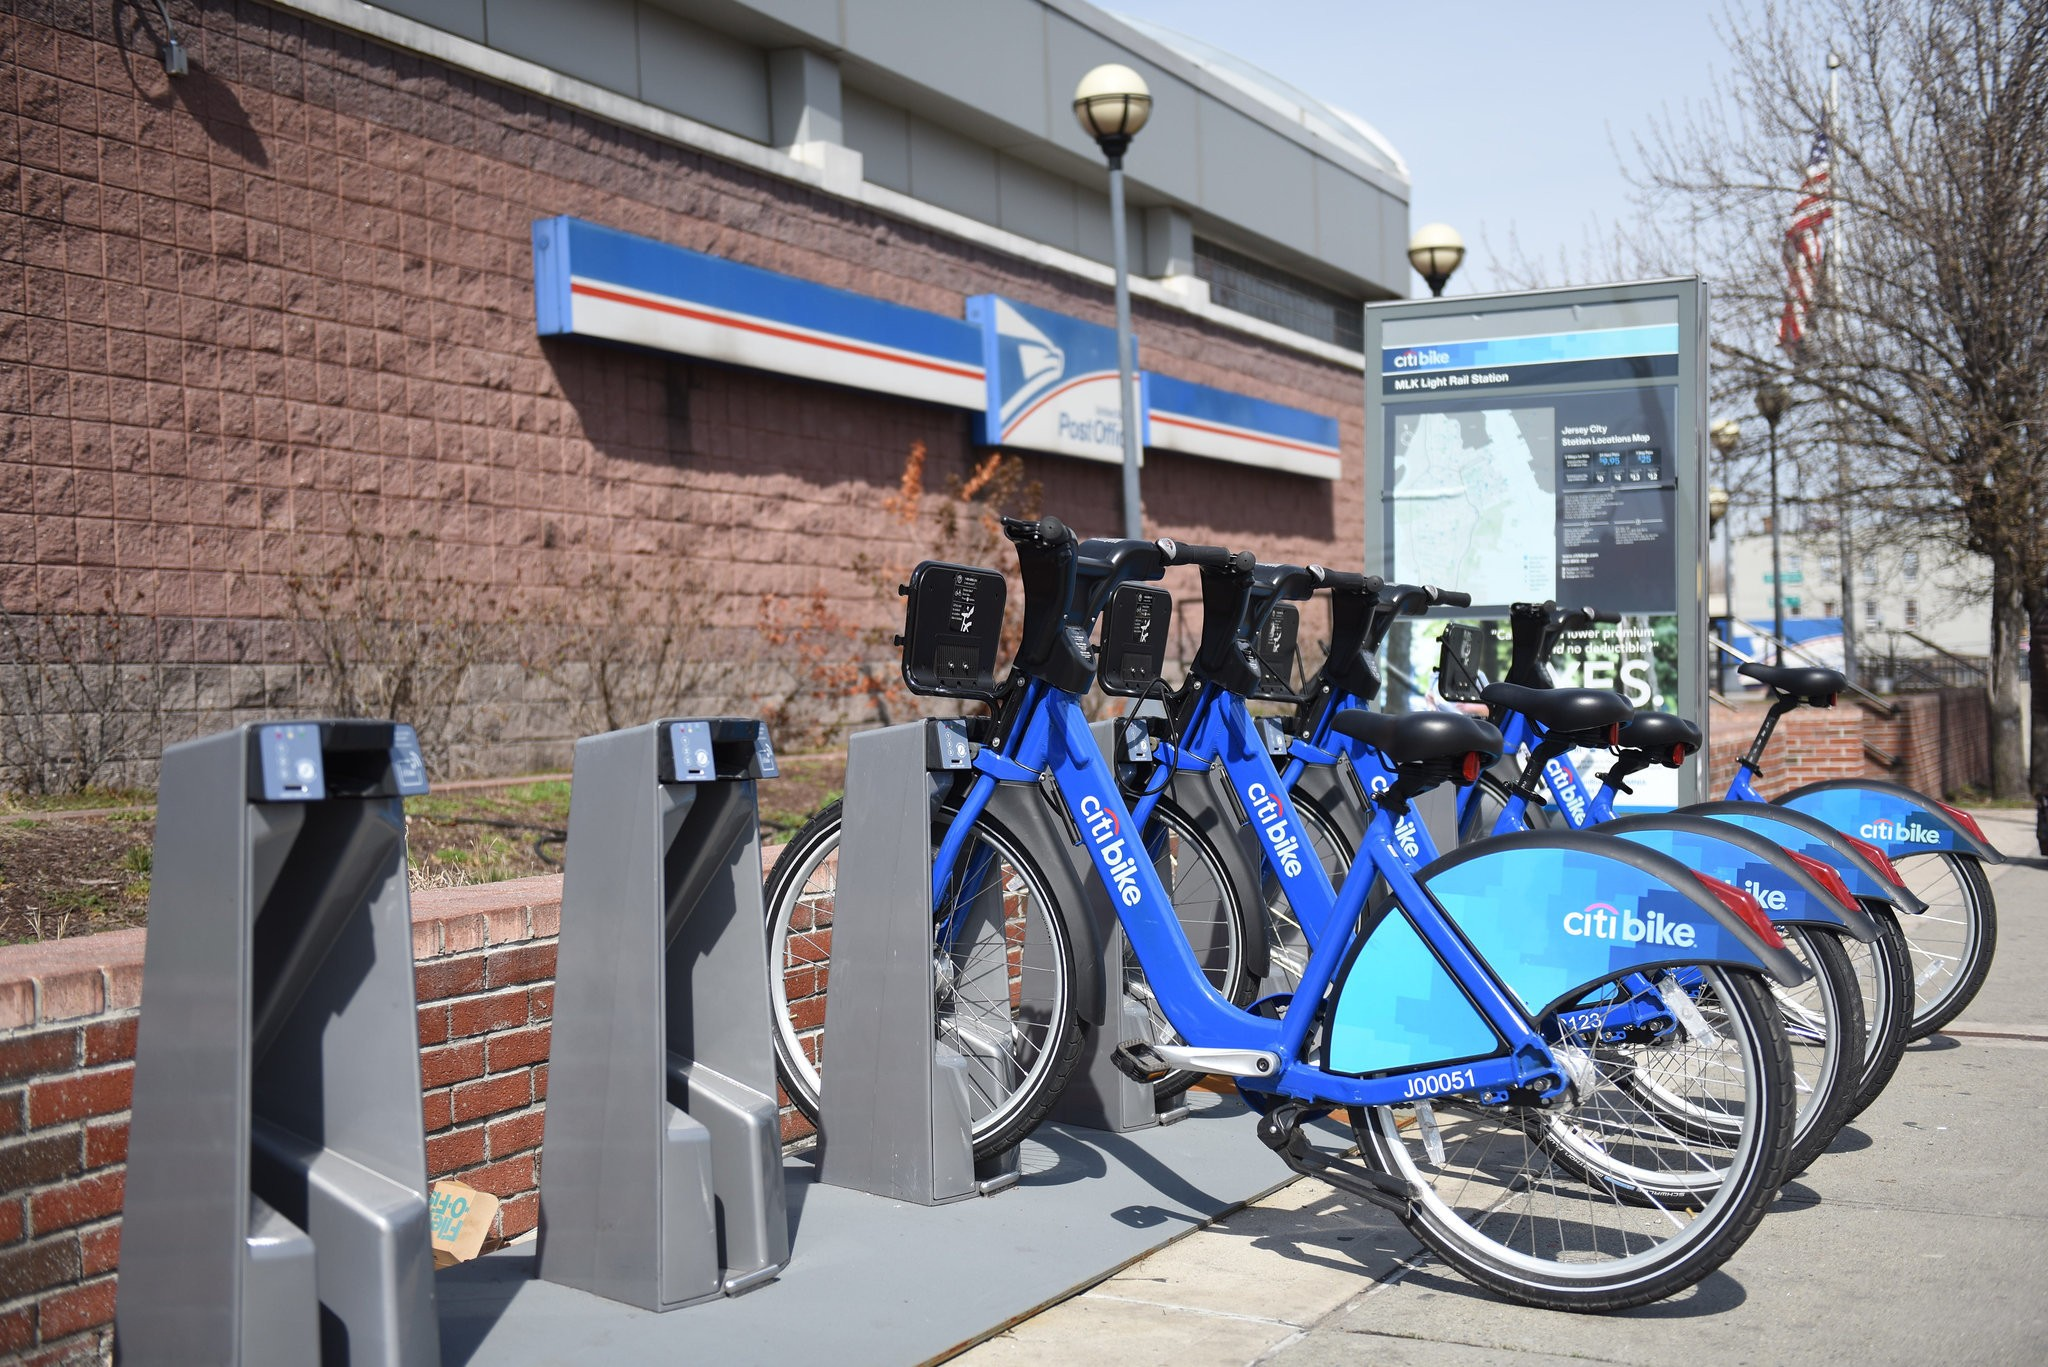
\includegraphics[height=137px]{Immagini/4. Caso di studio/Introduzione/Citi Bike}\label{Citi_Bike}}\quad
	\subfigure[]{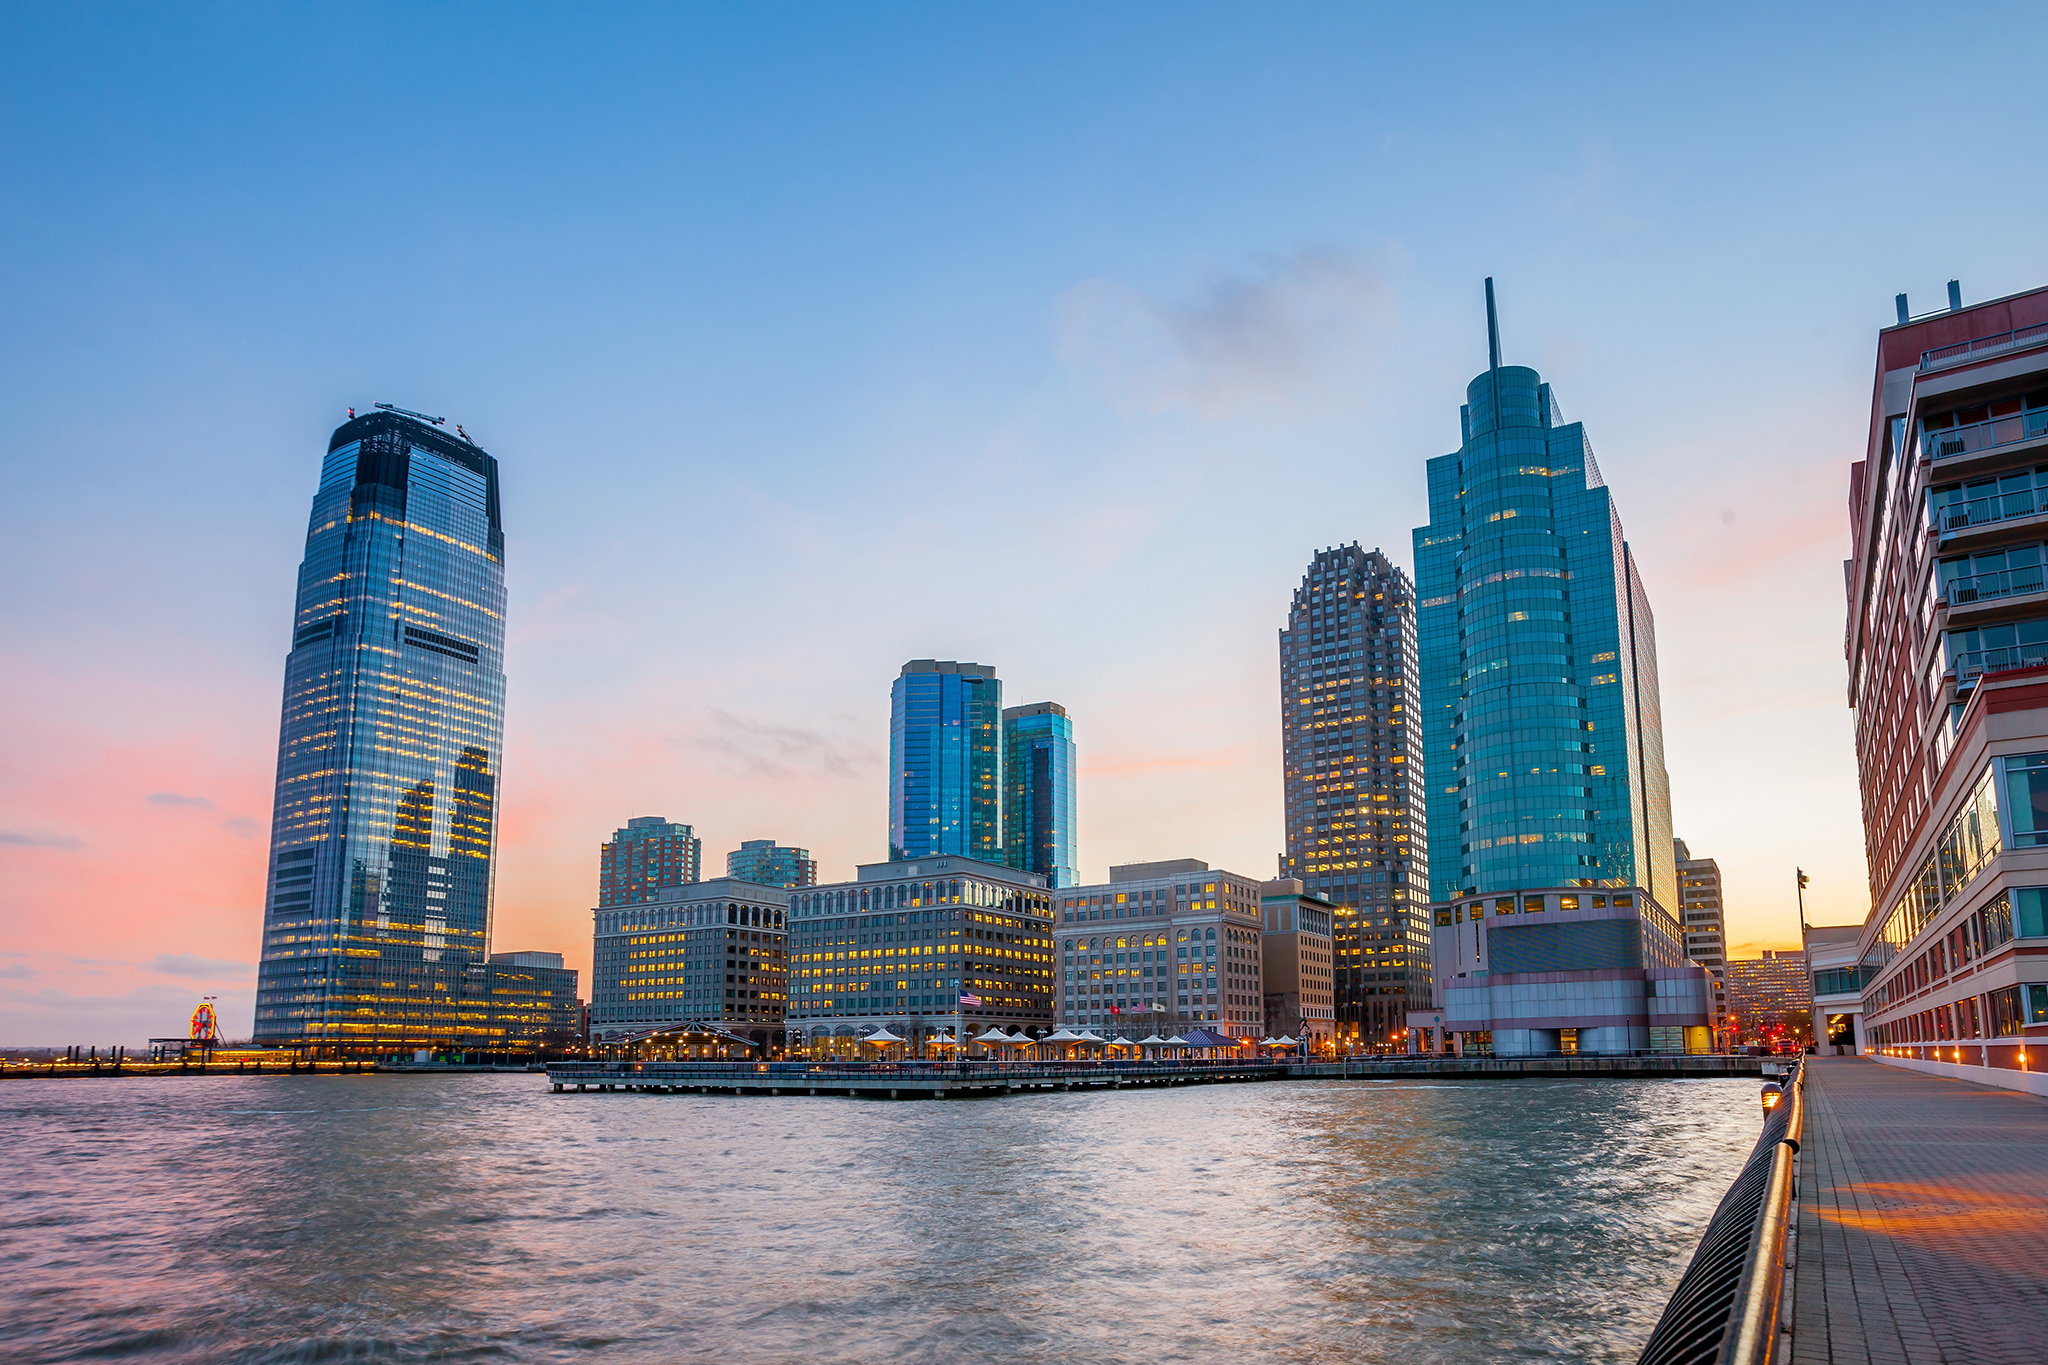
\includegraphics[height=137px]{Immagini/4. Caso di studio/Introduzione/Veduta Jersey City}\label{veduta_Jersey_City}}\quad
	\caption[Punto di ritiro delle biciclette e veduta del quartiere Jersey]{punto di ritiro delle biciclette gestito da Citi Bike (a) e veduta del quartiere Jersey, New York City (b).}
	\label{presentazione_Jersey_City}
\end{figure}

\section[Stato dell'arte]{Stato dell'arte}
Nelle città di tutto il mondo, l'inquinamento atmosferico rappresenta una sfida sempre più urgente e complessa. Samantha Burgess, Deputy Director del Copernicus Climate Change Service, ha affermato che il 2023 non solo è stato l'anno più caldo mai registrato, ma è anche il primo in cui tutti i giorni le temperature hanno fatto registrare valori superiori di almeno \SI{1}{\degreeCelsius} rispetto al periodo preindustriale~[\ref{sitografia_capitolo_4}].
\par L'aumento del traffico veicolare, in particolare, contribuisce in modo significativo alla diffusione di gas nocivi (es. CO$_2$ ed NO$_\text{X}$) e particolato nell'aria (es. PM\num{2.5} e PM\num{10}), compromettendo la salute pubblica e l'ambiente. In questo contesto, il bike sharing emerge come una soluzione innovativa e sostenibile per affrontare l'inquinamento urbano. Attraverso la condivisione delle biciclette, questo sistema offre un'alternativa efficace al trasporto privato a motore, riducendo le emissioni di gas serra, i consumi energetici e migliorando la qualità dell'aria nelle città~[\cite{paper_bike_sharing_e_ambiente}].
\par Per modellare il fenomeno del bike sharing le condizioni del tempo atmosferico risultano essere appropriate. Infatti, le variabili meteorologiche come pioggia, temperatura e vento, giocano un ruolo cruciale nel determinare la frequenza e la disponibilità delle biciclette per gli utenti, nonché la percezione stessa dell'attrattività del bike sharing come mezzo di trasporto. Inoltre, risulta interessante capire se la vicinanza di un punto di ritiro dalla più vicina fermata del treno o metropolitana incentiva l'utilizzo di quest'ultima piuttosto che della bicicletta, soprattutto in condizioni di maltempo~[\cite{paper_bike_sharing_e_meteo}].
\par In generale, anche gli aspetti urbanistici e demografici possono aiutare nella descrizione del fenomeno. Infatti, la densità abitativa, la disposizione delle infrastrutture ciclabili, la distribuzione della popolazione, la vicinanza ad alberghi e ai punti di interesse possono influenzare l'adozione della bicicletta a noleggio come mezzo di trasporto urbano~[\cite{paper_bike_sharing_e_popolazione}].
\par Infine, anche gli eventi straordinari possono avere un impatto significativo sul comportamento degli utenti e sulla dinamica del sistema. Uno di questi eventi straordinari è rappresentato dal lockdown imposto a causa della pandemia di COVID-\num{19}. Il lockdown ha comportato una serie di cambiamenti radicali nelle abitudini di spostamento delle persone, con effetti tangibili sull'utilizzo del bike sharing nelle metropoli di tutto il mondo. Pertanto, è essenziale comprendere come la chiusura obbligata abbia influenzato il fenomeno in oggetto, considerando sia gli aspetti legati alla riduzione del trasporto pubblico che quelli associati alla promozione di modalità di spostamento individuali e sicure~[\cite{paper_bike_sharing_e_covid}].
\par In questo contesto, l'impiego di un modello spazio-temporale funzionale si presenta come una soluzione promettente per catturare la dinamica complessa che governa il noleggio e scambio di biciclette. Tale famiglia di modelli consente di considerare non solo le variazioni spaziali dell'utilizzo delle biciclette all'interno di una città, ma anche come queste variazioni si evolvono nel tempo, consentendo una comprensione più approfondita dei pattern di utilizzo e dei fattori che li influenzano. Altresì, la modellazione funzionale permette di descrivere l'evoluzione oraria del numero di ritiri durante il giorno. Infatti, quest'ultimo non rimane costante nel corso della giornata, ma presenta un andamento periodico che raggiunge i propri massimi nelle ore di punta. I trend periodici, inoltre, sono influenzati dalla tipologia di giorno, ovvero feriale o weekend (figura~\ref{trend_paper_Otto}), quindi tenere in considerazione quest'aspetto nella modellazione è fondamentale~[\cite{paper_bike_sharing_Otto}].

\begin{figure}[htpb]
	\centering
	\subfigure[]{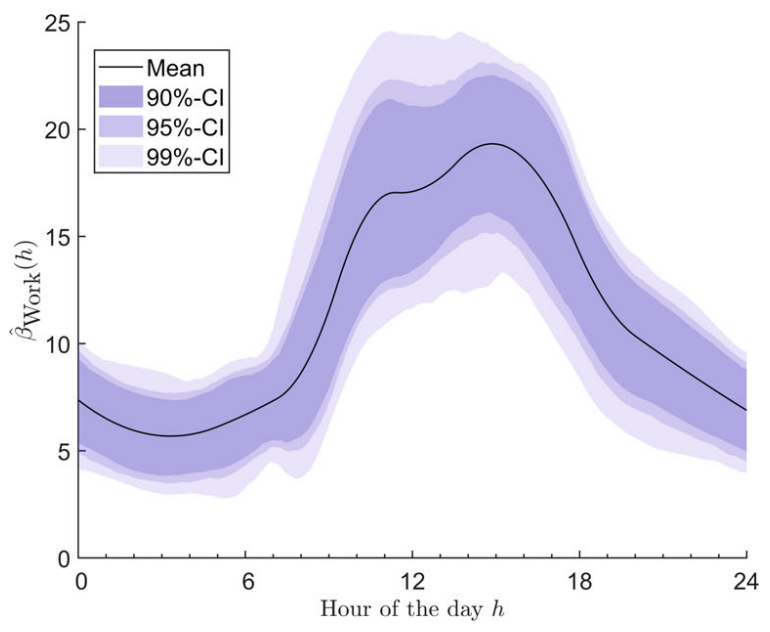
\includegraphics[height=156px]{Immagini/4. Caso di studio/Stato dell'arte/Trend_feriale}\label{trend_feriale}}\quad
	\subfigure[]{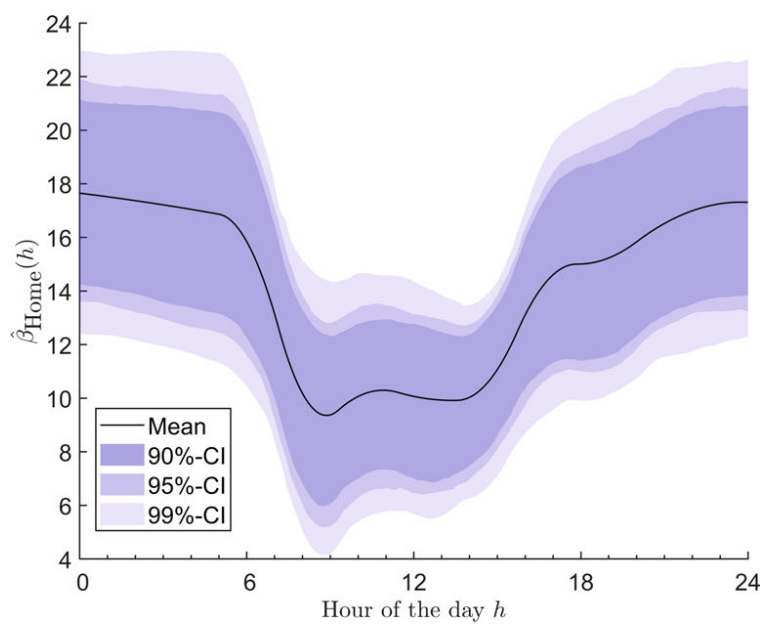
\includegraphics[height=156px]{Immagini/4. Caso di studio/Stato dell'arte/Trend_festivo}\label{trend_festivo}}\quad
	\caption[Confronto tra l'andamento orario del numero medio di ritiri nei giorni feriali e nei weekend a Helsinki]{confronto tra l'andamento orario del numero medio di ritiri di biciclette nei giorni feriali (a) e nei weekend (b) nella città di Helsinki, Finlandia.}
	\label{trend_paper_Otto}
\end{figure}

\section[Ricerca e acquisizione dati]{Ricerca e acquisizione dei dati}
Di seguito sono riportate le sorgenti dei dati utilizzati nel caso di studio:
\begin{itemize}
	\item \textbf{dati riguardanti il bike sharing}: provengono dal sito web Kaggle~[\ref{sitografia_capitolo_4}] e contengono le informazioni sul noleggio di biciclette nel \num{2020} dell'azienda Citi Bile a Jersey City. Citi Bike è un sistema di bike sharing pubblico di proprietà privata che serve i distretti di New York City, nello specifico Bronx, Brooklyn, Manhattan e Queens, oltre a Jersey City;
	\item \textbf{dati meteorologici}: contengono le serie storiche delle variabili meteorologiche più significative per la città di New York nel \num{2020}. Il provider di questi dati è Visual Crossing~[\ref{sitografia_capitolo_4}], un fornitore che offre una vasta gamma di soluzioni per l'accesso ai dati meteorologici storici e in tempo reale, nonché per la generazione di previsioni meteo;
	\item \textbf{dati inerenti le stazioni del treno/metropolitana}: dopo aver recuperato i nomi delle stazioni del treno e della metropolitana dalla mappa dei mezzi pubblici newyorkesi~[\ref{sitografia_capitolo_4}], le loro coordinate sono state reperite tramite Google Maps;
	\item \textbf{dati demografici}: il fornitore è il SEDAC~[\ref{sitografia_capitolo_4}] (Socioeconomic Data and Applications Center), un data center che fa parte del programma Earth Observing System Data and Information System (EOSDIS) della NASA. La missione principale dell'ente è quella di fornire accesso a dati socioeconomici e ambientali globali, nonché a strumenti e risorse per facilitare la ricerca e la comprensione dei cambiamenti ambientali e delle dinamiche sociali.
	\item \textbf{dati riguardanti i giorni di festività e di lockdown}: per i primi è stato fatto riferimento al sito web OfficeHolidays~[\ref{sitografia_capitolo_4}], mentre per i secondi a Wikipedia~[\ref{sitografia_capitolo_4}].
\end{itemize}
Da sottolineare, infine, che sono state processate le sole variabili d'interesse per il caso di studio; nello specifico è stato applicato un raggruppamento su base oraria, ove necessario.

\section[Descrizione del dataset]{Descrizione del dataset}
Di seguito sono riportate e descritte le variabili che compongono il dataset utilizzato per il caso di studio. Nello specifico la variabile dipendente $y(\mathbf{s}, l, t|\mathcal{S})$ è il numero di ritiri in una data ora $l$, in uno specifico giorno $t$, presso una determinata stazione di scambio di biciclette $\mathbf{s}$. Invece, le covariate possono essere suddivise in:
\begin{itemize}
	\item \textbf{variabili meteorologiche} $\mathbf{x}_{meteo}(t)$;
	\item \textbf{variabili spaziali} $\mathbf{x}_{spazio}(\mathbf{s})$;
	\item \textbf{variabili dummy} $\mathbf{x}_{dummy}(t)$.
\end{itemize}
Per completezza:
\begin{itemize}
	\item il numero di stazioni $n$ è pari a \num{51};
	\item il numero massimo di osservazioni disponibili per il dominio funzionale (orario) è \num{24};
	\item l'analisi è stata condotta su dati facenti riferimento all'anno \num{2020}, quindi $T=366$.
\end{itemize}
Infine, nel dataset non sono presenti record mancati.

\subsection[Numero di ritiri]{Variabile dipendente}
In figura~\ref{mappe_ritiri_per_stagione} si può osservare come il numero medio di ritiri giornaliero di biciclette presso le stazioni della rete di bike sharing cambi da stagione a stagione. Questa variazione è influenzata da diversi fattori legati alle condizioni meteorologiche, agli schemi di mobilità delle persone e alle attività ricreative. In estate, quando le giornate sono più lunghe e il clima è più gradevole, si verifica un generale aumento dell'utilizzo della bicicletta, figura~\ref{mappa_ritiri_estate}; le persone sono più propense a utilizzarla per spostarsi o fare gite. In autunno, invece, il numero di noleggi diminuisce leggermente poiché le giornate diventano più corte e il clima meno favorevole, figura~\ref{mappa_ritiri_autunno}. In inverno il numero medio di ritiri giornaliero tende a essere il più basso dell'anno, figura~\ref{mappa_ritiri_inverno}; le condizioni meteorologiche avverse, come il freddo, la pioggia e la neve, rendono meno attraente l'utilizzo della bicicletta. La primavera, infine, rispecchia la straordinarietà del \num{2020}; il lockdown ha limitato gli spostamenti dei cittadini newyorkesi, quindi l'utilizzo della bicicletta ha subito un brusco calo. Da notare, inoltre, l'assenza di uniformità nell'utilizzo delle stazioni; quelle situate nel centro del quartiere Jersey vengono sfruttate maggiormente rispetto ai punti di scambio periferici.
\par Infine, l'andamento orario del numero medio di noleggi in figura~\ref{ritiri_giornalieri_orari} conferma quanto detto precedentemente. Da sottolineare anche la presenza di picchi di utilizzo in concomitanza delle ore di punta.

\begin{figure}[htpb]
	\centering
	\subfigure[]{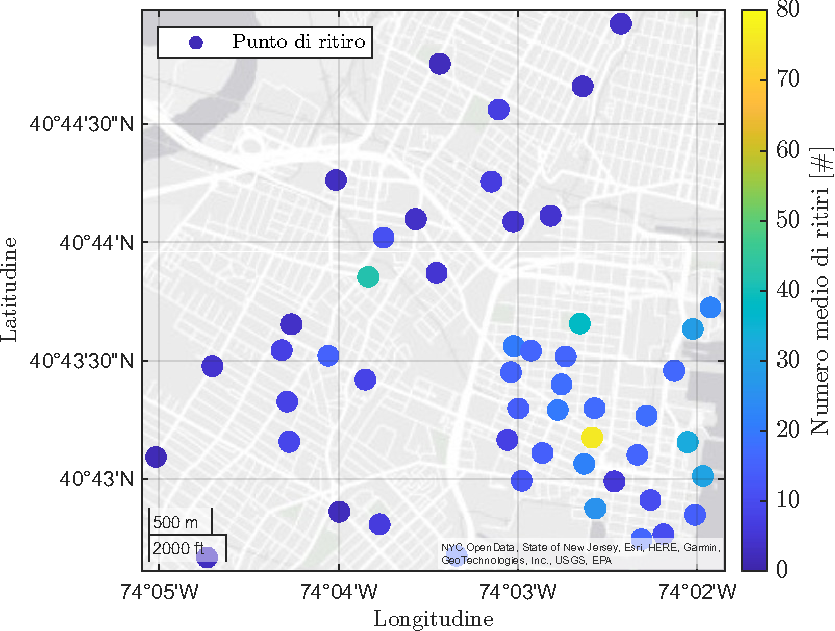
\includegraphics[height=156px]{Immagini/4. Caso di studio/Mappe/Mappa ritiri, inverno}\label{mappa_ritiri_inverno}}\quad
	\subfigure[]{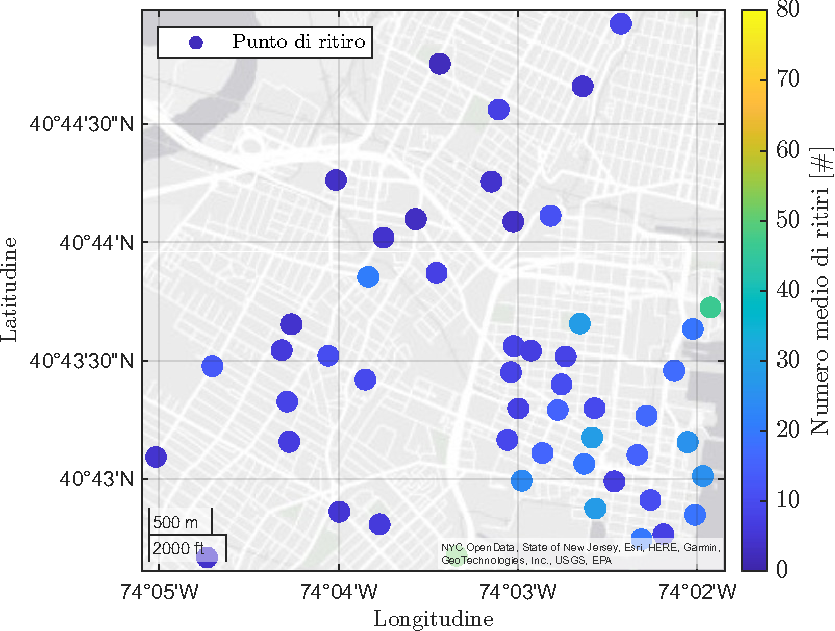
\includegraphics[height=156px]{Immagini/4. Caso di studio/Mappe/Mappa ritiri, primavera}\label{mappa_ritiri_primavera}}\quad
	\subfigure[]{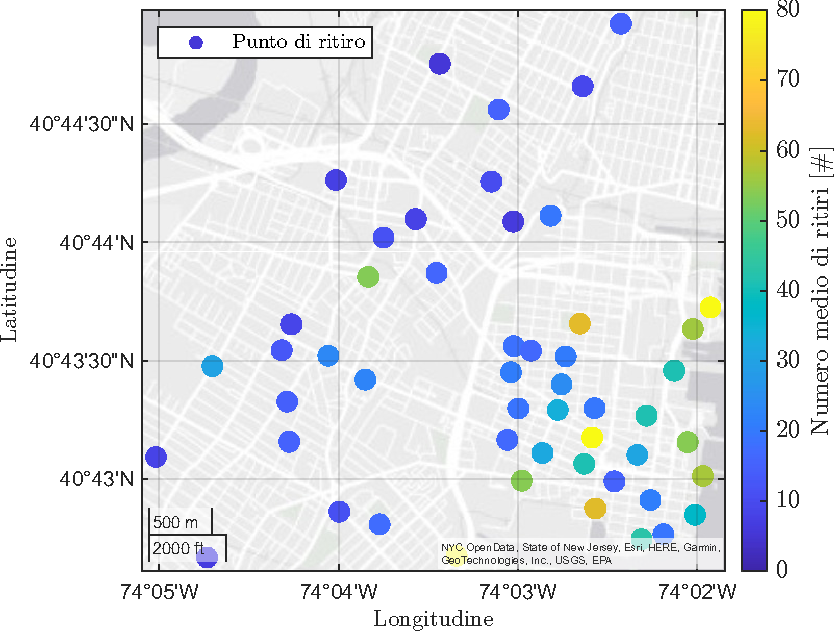
\includegraphics[height=156px]{Immagini/4. Caso di studio/Mappe/Mappa ritiri, estate}\label{mappa_ritiri_estate}}\quad
	\subfigure[]{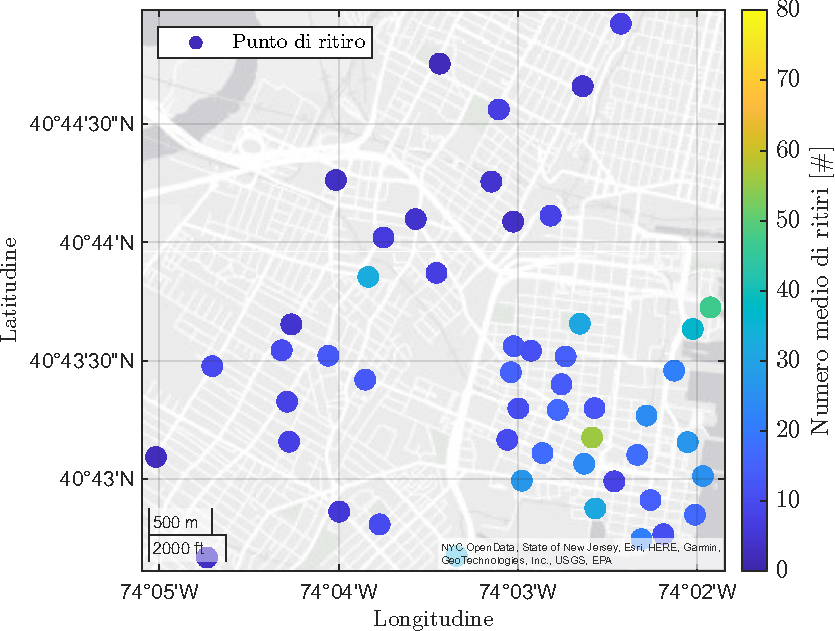
\includegraphics[height=156px]{Immagini/4. Caso di studio/Mappe/Mappa ritiri, autunno}\label{mappa_ritiri_autunno}}\quad
	\caption[Distribuzione nel numero medio di ritiri giornaliero presso le stazioni al variare della stagione]{distribuzione nel numero medio di ritiri giornaliero presso le \num{51} stazioni di scambio in inverno (a), in primavera (b), in estate (c) e in autunno (d).}
	\label{mappe_ritiri_per_stagione}
\end{figure}

\begin{figure}[htpb]
	\centering
	\subfigure[]{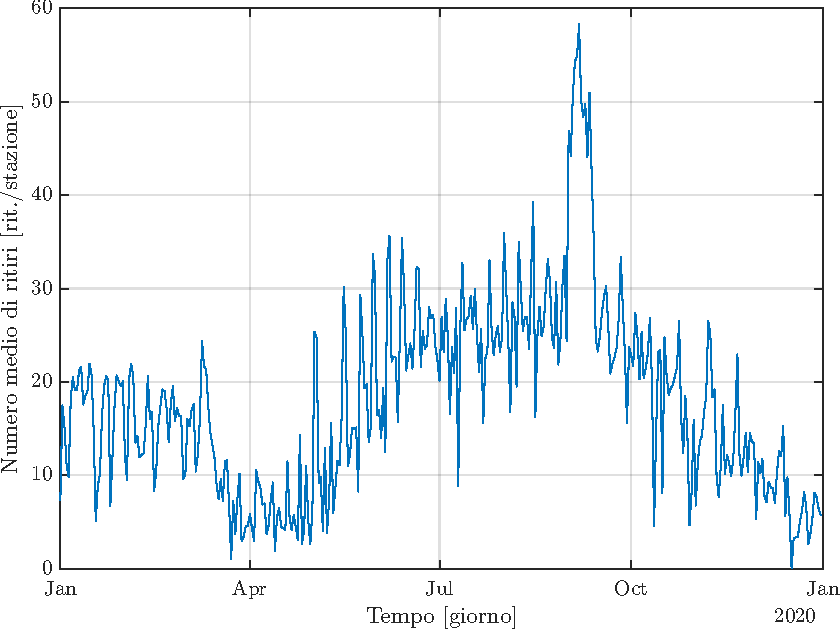
\includegraphics[height=156px]{Immagini/4. Caso di studio/Serie storiche/Ritiri giornalieri}}\quad
	\subfigure[]{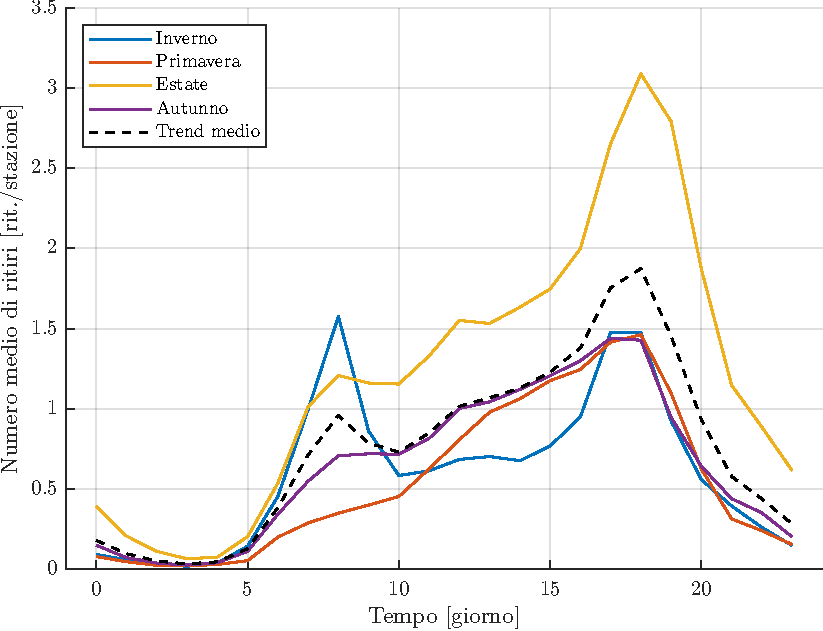
\includegraphics[height=156px]{Immagini/4. Caso di studio/Serie storiche/Ritiri orari}}\quad
	\caption[Andamento giornaliero e orario del numero medio di ritiri al variare della stagione]{andamento giornaliero (a) e orario (b) del numero medio di ritiri al variare della stagione.}
	\label{ritiri_giornalieri_orari}
\end{figure}

\subsection[Variabili meteorologiche]{Variabili meteorologiche}
Le covariate meteorologiche che sono state utilizzate per l'analisi sono:
\begin{itemize}
	\item la \textbf{temperatura percepita}  [\unit{\degreeCelsius}];
	\item la \textbf{pioggia} [\unit{\milli\meter}];
	\item la \textbf{visibilità orizzontale} [\unit{\kilo\meter}];
	\item la \textbf{velocità del vento} [\unit{\kilo\meter/\hour}];
	\item la \textbf{copertura nuvolosa} [\unit{\percent}].
\end{itemize}
Da sottolineare che le variabili sopracitate sono spazio-invarianti e orarie, ovvero sono conseguenza della media eseguita sui campioni rilevati nell'ora da una stazione meteorologica di New York. Inoltre, nella tabella~\ref{statistiche_variabili_meteo} sono riportate le principali statistiche delle covariate in questione; degne di nota la scarsa variabilità della visibilità orizzontale e l'elevata dispersione della copertura nuvolosa nel \num{2020}.

\begin{table}[htp]
	\centering
	\renewcommand\arraystretch{1.5}
	\begin{tabular}{c|c|c|c|c|c|c|c|c}
		\hline
		\textit{Variabile} & \textit{UM} & \textit{Min.} & \textit{Media} & \textit{Med.} & \textit{Mas.} & \textit{Dev.} & \textit{Simm.}  & \textit{Curt.} \\
		\hline
		\textbf{Temp. percep.} & \unit{\degreeCelsius} & \num{-7.66} & \num{13.80} & \num{13.93} & \num{33.33} & \num{9.80} & \num{-0.04} & \num{1.96} \\
		\hline
		\textbf{Pioggia} & \unit{\milli\meter} & \num{0} & \num{1.11} & \num{0} & \num{31.03} & \num{3.44} & \num{5.42} & \num{38.86} \\
		\hline
		\textbf{Visibilità} & \si{\kilo\meter} & \num{6.48} & \num{15.28} & \num{15.99} & \num{16} & \num{1.54} & \num{-2.99} & \num{12.71} \\
		\hline
		\textbf{Vel. del vento} & \si{\kilo\meter/\hour} & \num{4.09} & \num{10.96} & \num{9.81} & \num{27.95} & \num{4.49} & \num{1.34} & \num{4.91} \\
		\hline
		\textbf{Copert. nuvol.} & \si{\percent} & \num{0.08} & \num{39.45} & \num{37.29} & \num{100} & \num{29.71} & \num{0.36} & \num{1.96} \\
		\hline
	\end{tabular}
	\caption[Statistiche principali riguardanti le variabili meteorologiche]{statistiche principali riguardanti le variabili meteorologiche. Per la pioggia è stata eseguita la somma giornaliera.}
	\label{statistiche_variabili_meteo}
\end{table}

\par Infine, è possibile osservare in figura~\ref{ritiri_vs_temperatura} la correlazione positiva esistente tra il numero medio di ritiri giornaliero e la temperatura percepita, mentre in figura~\ref{ritiri_vs_pioggia} l'impatto negativo nei confronti dello stesso da parte della pioggia; nei giorni uggiosi i cittadini newyorkesi prediligono mezzi di trasporto alternativi alla bicicletta.
\par Per gli istogrammi, i box-plot e ulteriori grafici si rimanda all'appendice.

\begin{figure}[htpb]
	\centering
	\subfigure[]{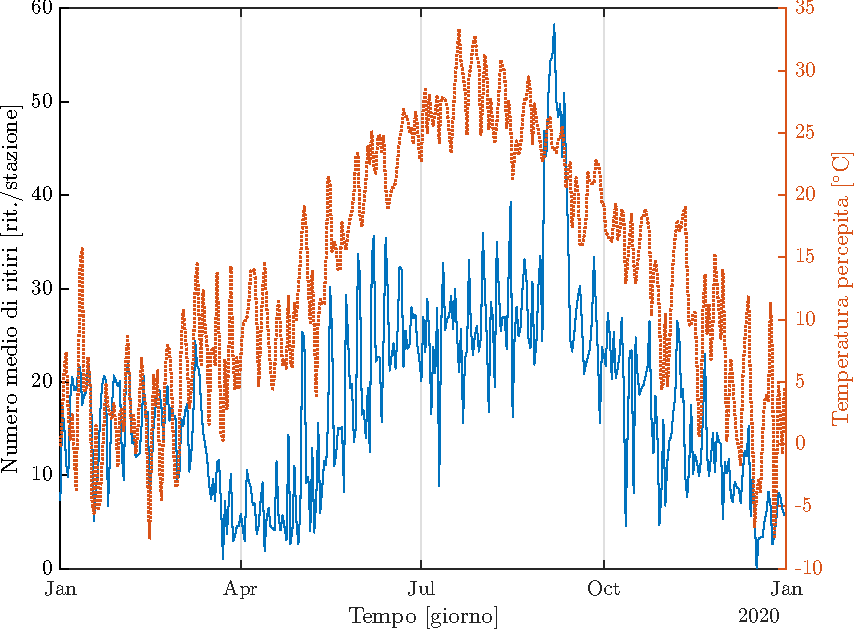
\includegraphics[height=152px]{Immagini/4. Caso di studio/Serie storiche/Ritiri giornalieri e temperatura percepita}\label{ritiri_vs_temperatura}}\quad
	\subfigure[]{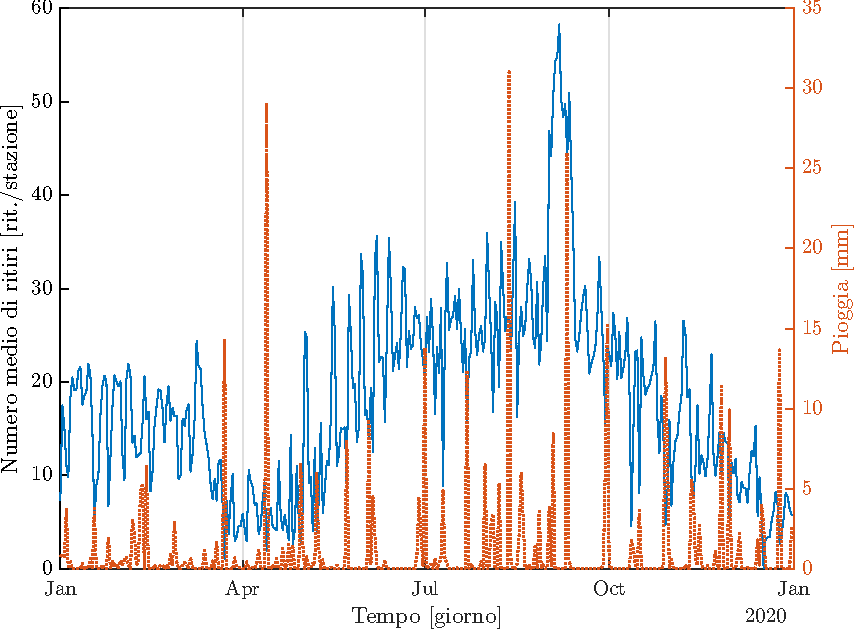
\includegraphics[height=152px]{Immagini/4. Caso di studio/Serie storiche/Ritiri giornalieri e pioggia}\label{ritiri_vs_pioggia}}\quad
	\caption[Confronto tra il numero medio di noleggi giornaliero, la temperatura percepita e la pioggia]{confronto tra il numero medio di noleggi giornaliero, la temperatura percepita (a) e la pioggia (b).}
	\label{ritiri_vs_variabili_meteo}
\end{figure}

\subsection[Variabili spaziali]{Variabili spaziali}
In questa categoria ricadono:
\begin{itemize}
	\item la \textbf{distanza dalla stazione del treno\footnote{o fermata della metropolitana poiché Jersey City è servita da entrambi i mezzi di trasporto pubblico.} più vicina} [\unit{\kilo\meter}];
	\item la \textbf{densità demografica} nella zona alla quale appartiene il punto di ritiro [ab./\unit{\kilo\meter\squared}].
\end{itemize}
Da sottolineare che queste covariate sono spazio-varianti e tempo-invarianti.
\par In figura~\ref{mappa_stazioni_metro} è rappresentata la distanza di ciascun punto di interscambio dalla stazione ferroviaria più vicina. Si osserva una densa concentrazione sia di stazioni ferroviarie che di punti di ritiro delle biciclette nel centro del quartiere, densità che diminuisce man mano che ci si sposta verso le zone limitrofe. Riguardo alla densità demografica, come evidenziato nella figura~\ref{mappa_densita_demografica}, si può notare una distribuzione omogenea su Jersey City. Questa osservazione è supportata dalla ridotta deviazione standard (\num{4278} ab./\unit{\kilo\meter\squared}) della covariata in oggetto (tabella~\ref{statistiche_variabili_spaziali}).

\begin{figure}[htpb]
	\centering
	\subfigure[]{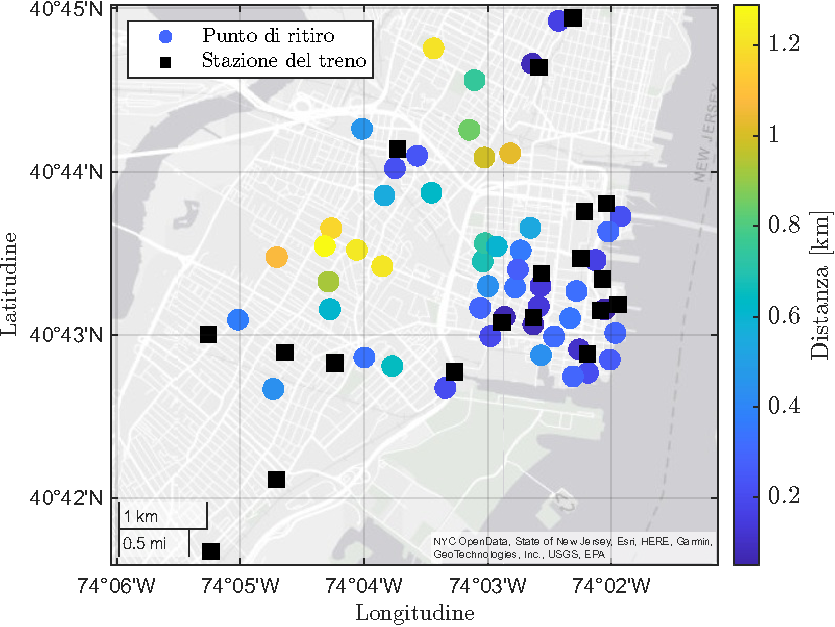
\includegraphics[height=152px]{Immagini/4. Caso di studio/Mappe/Mappa punti ritiro e stazioni treno}\label{mappa_stazioni_metro}}\quad
	\subfigure[]{\includegraphics[height=161px]{Immagini/4. Caso di studio/Mappe/Mappa punti ritiro e densità abitativa}\label{mappa_densita_demografica}}\quad
	\caption[Mappe delle distanze dei punti di interscambio dalla stazione ferroviaria più vicina e della densità abitativa nei pressi dei punti di ritiro]{mappe delle distanze dei punti di interscambio dalla stazione ferroviaria più vicina (a) e della densità abitativa nei pressi dei punti di ritiro (b).}
	\label{mappe_variabili_spaziali}
\end{figure}

\begin{table}[htpb]
	\centering
	\renewcommand\arraystretch{1.5}
	\begin{tabular}{c|c|c|c|c|c|c|c|c}
		\hline
		\textit{Variabile} & \textit{UM} & \textit{Min.} & \textit{Media} & \textit{Med.} & \textit{Mas.} & \textit{Dev.} & \textit{Simm.}  & \textit{Curt.} \\
		\hline
		\textbf{Dist. stazione} & \unit{\kilo\meter} & \num{0.05} & \num{0.49} & \num{0.35} & \num{1.29} & \num{0.36} & \num{0.89} & \num{2.64} \\
		\hline
		\textbf{Dens. dem.} & $\frac{\text{ab.}}{\unit{\kilo\meter\squared}}$ & \num{897} & \num{12215} & \num{11843} & \num{22834} & \num{4278} & \num{-0.15} & \num{2.80} \\
		\hline
	\end{tabular}
	\caption[Statistiche principali riguardanti le variabili spaziali]{statistiche principali riguardanti le variabili spaziali.}
	\label{statistiche_variabili_spaziali}
\end{table} 

\subsection[Variabili dummy]{Variabili dummy}
Alla luce dei risultati ottenuti in~\cite{paper_bike_sharing_Otto}, non solo le condizioni meteorologiche e le covariate spaziali influenzano la domanda giornaliera di noleggi, ma anche altri fattori possono fornire il proprio contributo. In particolare:
\begin{itemize}
	\item il \textbf{lockdown} dovuto alla pandemia di COVID-\num{19};
	\item la successiva \textbf{euforia} dovuta al ritorno alla vita quotidiana dopo mesi trascorsi in isolamento;
	\item i \textbf{weekend} e le \textbf{festività} federali\footnote{giorno di festa ufficialmente riconosciuto a livello federale dal governo degli Stati Uniti.}.
\end{itemize}
Questi eventi sono stati modellati utilizzando \num{3} distinte variabili categoriche binarie (covariate dummy).
\par Infine, la figura~\ref{ritiri_vs_dummy} conferma che, durante la primavera, il numero ridotto di noleggi coincide con il periodo di lockdown, mentre nei weekend si osserva una generale riduzione dell'utilizzo della bicicletta, a dimostrazione che il servizio di bike sharing viene essenzialmente sfruttato nei giorni feriali, probabilmente per i consueti spostamenti lavorativi.

\begin{figure}[htpb]
	\centering
	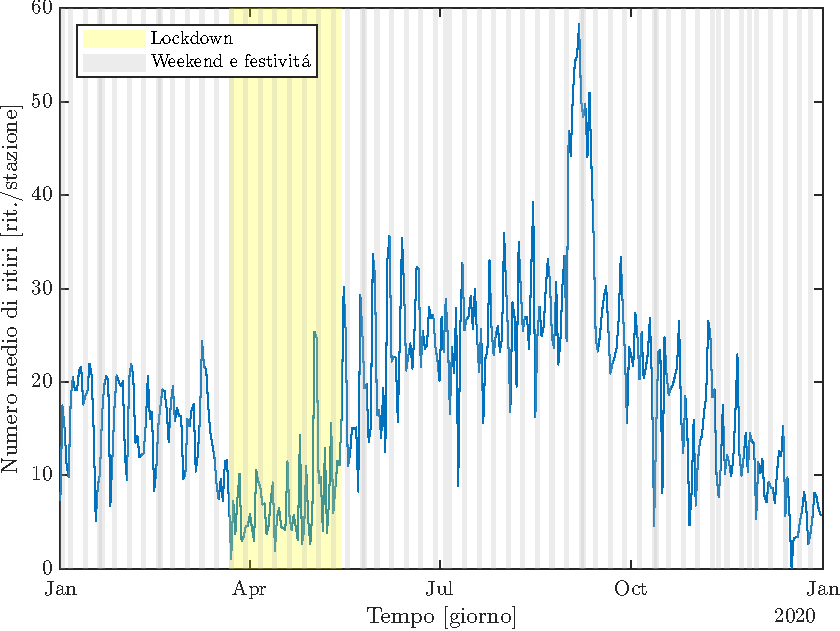
\includegraphics[height=170px]{Immagini/4. Caso di studio/Serie storiche/Ritiri giornalieri e dummy}
	\caption[Confronto tra il numero medio di prelievi giornaliero, il periodo di lockdowwn, i weekend e le festività federali.]{confronto tra il numero medio di prelievi giornaliero, il periodo di lockdowwn, i weekend e le festività federali.}
	\label{ritiri_vs_dummy}
\end{figure}

\section{Sitografia}
\label{sitografia_capitolo_4}
Di seguito sono riportati i riferimenti alle risorse citate in questo capitolo:
\begin{itemize}
	\item \textit{https://climate.copernicus.eu/copernicus-2023-hottest-year-record};
	\item \textit{https://www.kaggle.com/datasets/vineethakkinapalli/citibike-bike-sharingnewyork-cityjan-to-apr-2021};
	\item \textit{https://www.visualcrossing.com/weather-api};
	\item \textit{https://stewartmader.com/subwaynynj/};
	\item \textit{https://sedac.ciesin.columbia.edu/data/set/gpw-v4-population-density-adjusted-to-2015-unwpp-country-totals-rev11};
	\item \textit{https://www.officeholidays.com/countries/usa/new-york/2020};
	\item \textit{https://en.wikipedia.org/wiki/COVID-19\_pandemic\_in\_New\_York\_City}.
\end{itemize}

	\chapter[Conclusioni]{Conclusioni}

Alla luce dei risultati ottenuti, il presente studio evidenzia il valore aggiunto del nuovo modello proposto nel campo della modellazione funzionale spazio-temporale come un'evoluzione rispetto al modello f-HDGM. Una delle distinzioni chiave di questo lavoro è l'introduzione del parametro di interazione spaziale $\rho$, il quale consente di affrontare situazioni e dinamiche in cui esiste interazione tra i punti di misura, un aspetto non considerato dal modello padre.
\par È importante notare che una delle limitazioni riguarda il processo di stima del nuovo parametro utilizzato nel modello proposto. Sebbene sia stata impiegata una metodologia affidabile come la cross-validazione per stimare il suo valore, è necessario sottolineare che tale approccio richiede notevoli risorse computazionali; questa necessità potrebbe costituire un ostacolo pratico per alcuni utenti, specialmente in contesti nei quali le risorse computazionali sono limitate. Per superare questo ostacolo, si rende necessaria la modifica dell'algoritmo EM affinché sia in grado di minimizzare anche la funzione $m(\rho)$, equazione~\ref{eq_f_rho}. Come anticipato nella sezione~\ref{metodologia}, la sua implementazione in D-STEM è già stata avviata, tuttavia richiede ancora un periodo di ricerca e sviluppo per poter rispondere ad alcuni quesiti ancora aperti. Innanzitutto, un aspetto cruciale risiede nella verifica dell'identificabilità di $\rho$, ossia capire se esso può essere stimato congiuntamente agli altri parametri $\boldsymbol{\theta}$, espressione~\ref{parametri_fp_HDGM}. In particolare, la stima di $\rho$ potrebbe andare in conflitto con quella di $\boldsymbol{\lambda}$ poiché entrambi vengono identificati tramite l'ottimizzazione numerica. Se ciò dovesse concretizzarsi, allora sarà opportuno stimare uno solo dei due parametri alla volta, tenendo fisso il restante. Dopodiché, un altro fattore da attenzionare riguarda l'inizializzazione di $\rho$. Essendo $m(\rho)$ una funzione non convessa, senza un'opportuna scelta del valore iniziale da assegnare al nuovo parametro si corre il rischio di identificare un minimo locale piuttosto che l'ottimo globale. Pertanto, per indirizzare l'ottimizzatore nella giusta direzione, è necessario avere un'idea a priori dell'ordine di grandezza di $\rho$, basandosi sulla conoscenza del dominio dello specifico caso di studio.
\par Infine, per quanto riguarda l'analisi svolta sul bike sharing, sarebbe interessante raffinare lo studio prendendo in esame un dataset pluriennale così da poter catturare anche la componente stagionale del fenomeno. Altresì, si potrebbero prendere in considerazioni delle variazioni metodologiche, per esempio eseguire un clustering dei punti di ritiro, a monte dell'analisi, ed eseguire così la stima di un modello spazio-temporale locale per ogni cluster. Ciò consentirebbe di rilassare un'importante assunzione fatta a priori, ossia che il parametro $\rho$ sia spazio-invariante.
	
	\cleardoublepage
	\phantomsection
	\addcontentsline{toc}{chapter}{Bibliografia}
	\bibliographystyle{apalike}
	\bibliography{Capitoli/Bibliografia.bib}

\end{document}